\documentclass[]{article}
\usepackage{lmodern}
\usepackage{amssymb,amsmath}
\usepackage{ifxetex,ifluatex}
\usepackage{fixltx2e} % provides \textsubscript
\ifnum 0\ifxetex 1\fi\ifluatex 1\fi=0 % if pdftex
  \usepackage[T1]{fontenc}
  \usepackage[utf8]{inputenc}
\else % if luatex or xelatex
  \ifxetex
    \usepackage{mathspec}
  \else
    \usepackage{fontspec}
  \fi
  \defaultfontfeatures{Ligatures=TeX,Scale=MatchLowercase}
\fi
% use upquote if available, for straight quotes in verbatim environments
\IfFileExists{upquote.sty}{\usepackage{upquote}}{}
% use microtype if available
\IfFileExists{microtype.sty}{%
\usepackage{microtype}
\UseMicrotypeSet[protrusion]{basicmath} % disable protrusion for tt fonts
}{}
\usepackage[margin=1in]{geometry}
\usepackage{hyperref}
\hypersetup{unicode=true,
            pdftitle={Premiers pas avec shiny\ldots{} et les packages de visualisation interactive},
            pdfauthor={B.Thieurmel, benoit.thieurmel@datastorm.fr},
            pdfborder={0 0 0},
            breaklinks=true}
\urlstyle{same}  % don't use monospace font for urls
\usepackage{color}
\usepackage{fancyvrb}
\newcommand{\VerbBar}{|}
\newcommand{\VERB}{\Verb[commandchars=\\\{\}]}
\DefineVerbatimEnvironment{Highlighting}{Verbatim}{commandchars=\\\{\}}
% Add ',fontsize=\small' for more characters per line
\usepackage{framed}
\definecolor{shadecolor}{RGB}{248,248,248}
\newenvironment{Shaded}{\begin{snugshade}}{\end{snugshade}}
\newcommand{\KeywordTok}[1]{\textcolor[rgb]{0.13,0.29,0.53}{\textbf{#1}}}
\newcommand{\DataTypeTok}[1]{\textcolor[rgb]{0.13,0.29,0.53}{#1}}
\newcommand{\DecValTok}[1]{\textcolor[rgb]{0.00,0.00,0.81}{#1}}
\newcommand{\BaseNTok}[1]{\textcolor[rgb]{0.00,0.00,0.81}{#1}}
\newcommand{\FloatTok}[1]{\textcolor[rgb]{0.00,0.00,0.81}{#1}}
\newcommand{\ConstantTok}[1]{\textcolor[rgb]{0.00,0.00,0.00}{#1}}
\newcommand{\CharTok}[1]{\textcolor[rgb]{0.31,0.60,0.02}{#1}}
\newcommand{\SpecialCharTok}[1]{\textcolor[rgb]{0.00,0.00,0.00}{#1}}
\newcommand{\StringTok}[1]{\textcolor[rgb]{0.31,0.60,0.02}{#1}}
\newcommand{\VerbatimStringTok}[1]{\textcolor[rgb]{0.31,0.60,0.02}{#1}}
\newcommand{\SpecialStringTok}[1]{\textcolor[rgb]{0.31,0.60,0.02}{#1}}
\newcommand{\ImportTok}[1]{#1}
\newcommand{\CommentTok}[1]{\textcolor[rgb]{0.56,0.35,0.01}{\textit{#1}}}
\newcommand{\DocumentationTok}[1]{\textcolor[rgb]{0.56,0.35,0.01}{\textbf{\textit{#1}}}}
\newcommand{\AnnotationTok}[1]{\textcolor[rgb]{0.56,0.35,0.01}{\textbf{\textit{#1}}}}
\newcommand{\CommentVarTok}[1]{\textcolor[rgb]{0.56,0.35,0.01}{\textbf{\textit{#1}}}}
\newcommand{\OtherTok}[1]{\textcolor[rgb]{0.56,0.35,0.01}{#1}}
\newcommand{\FunctionTok}[1]{\textcolor[rgb]{0.00,0.00,0.00}{#1}}
\newcommand{\VariableTok}[1]{\textcolor[rgb]{0.00,0.00,0.00}{#1}}
\newcommand{\ControlFlowTok}[1]{\textcolor[rgb]{0.13,0.29,0.53}{\textbf{#1}}}
\newcommand{\OperatorTok}[1]{\textcolor[rgb]{0.81,0.36,0.00}{\textbf{#1}}}
\newcommand{\BuiltInTok}[1]{#1}
\newcommand{\ExtensionTok}[1]{#1}
\newcommand{\PreprocessorTok}[1]{\textcolor[rgb]{0.56,0.35,0.01}{\textit{#1}}}
\newcommand{\AttributeTok}[1]{\textcolor[rgb]{0.77,0.63,0.00}{#1}}
\newcommand{\RegionMarkerTok}[1]{#1}
\newcommand{\InformationTok}[1]{\textcolor[rgb]{0.56,0.35,0.01}{\textbf{\textit{#1}}}}
\newcommand{\WarningTok}[1]{\textcolor[rgb]{0.56,0.35,0.01}{\textbf{\textit{#1}}}}
\newcommand{\AlertTok}[1]{\textcolor[rgb]{0.94,0.16,0.16}{#1}}
\newcommand{\ErrorTok}[1]{\textcolor[rgb]{0.64,0.00,0.00}{\textbf{#1}}}
\newcommand{\NormalTok}[1]{#1}
\usepackage{graphicx,grffile}
\makeatletter
\def\maxwidth{\ifdim\Gin@nat@width>\linewidth\linewidth\else\Gin@nat@width\fi}
\def\maxheight{\ifdim\Gin@nat@height>\textheight\textheight\else\Gin@nat@height\fi}
\makeatother
% Scale images if necessary, so that they will not overflow the page
% margins by default, and it is still possible to overwrite the defaults
% using explicit options in \includegraphics[width, height, ...]{}
\setkeys{Gin}{width=\maxwidth,height=\maxheight,keepaspectratio}
\IfFileExists{parskip.sty}{%
\usepackage{parskip}
}{% else
\setlength{\parindent}{0pt}
\setlength{\parskip}{6pt plus 2pt minus 1pt}
}
\setlength{\emergencystretch}{3em}  % prevent overfull lines
\providecommand{\tightlist}{%
  \setlength{\itemsep}{0pt}\setlength{\parskip}{0pt}}
\setcounter{secnumdepth}{5}
% Redefines (sub)paragraphs to behave more like sections
\ifx\paragraph\undefined\else
\let\oldparagraph\paragraph
\renewcommand{\paragraph}[1]{\oldparagraph{#1}\mbox{}}
\fi
\ifx\subparagraph\undefined\else
\let\oldsubparagraph\subparagraph
\renewcommand{\subparagraph}[1]{\oldsubparagraph{#1}\mbox{}}
\fi

%%% Use protect on footnotes to avoid problems with footnotes in titles
\let\rmarkdownfootnote\footnote%
\def\footnote{\protect\rmarkdownfootnote}

%%% Change title format to be more compact
\usepackage{titling}

% Create subtitle command for use in maketitle
\newcommand{\subtitle}[1]{
  \posttitle{
    \begin{center}\large#1\end{center}
    }
}

\setlength{\droptitle}{-2em}

  \title{Premiers pas avec shiny\ldots{} et les packages de visualisation
interactive}
    \pretitle{\vspace{\droptitle}\centering\huge}
  \posttitle{\par}
    \author{B.Thieurmel,
\href{mailto:benoit.thieurmel@datastorm.fr}{\nolinkurl{benoit.thieurmel@datastorm.fr}}}
    \preauthor{\centering\large\emph}
  \postauthor{\par}
    \date{}
    \predate{}\postdate{}
  
\usepackage{graphicx}
\usepackage{float}

\begin{document}
\maketitle

{
\setcounter{tocdepth}{2}
\tableofcontents
}
\section{Shiny : créer des applications web avec le logiciel
R}\label{shiny-creer-des-applications-web-avec-le-logiciel-r}

\textbf{Shiny} est un package \textbf{R} qui permet la création simple
d'applications web intéractives depuis le logiciel open-source
\textbf{R}.

\begin{itemize}
\tightlist
\item
  pas de connaissances \emph{web} nécessaires
\item
  le pouvoir de calcul de R et l'intéractivité du web actuel
\item
  pour créer des applications locales
\item
  ou partagées avec l'utilisation de \textbf{shiny-server},
  \textbf{shinyapps.io}, \textbf{shinyproxy}
\end{itemize}

\url{http://shiny.rstudio.com}

\url{http://www.shinyapps.io/}

\url{https://www.shinyproxy.io/}

\url{https://www.rstudio.com/products/shiny/shiny-server/}

Une application \textbf{shiny} nécessite un ordinateur/un serveur
éxécutant \textbf{R}

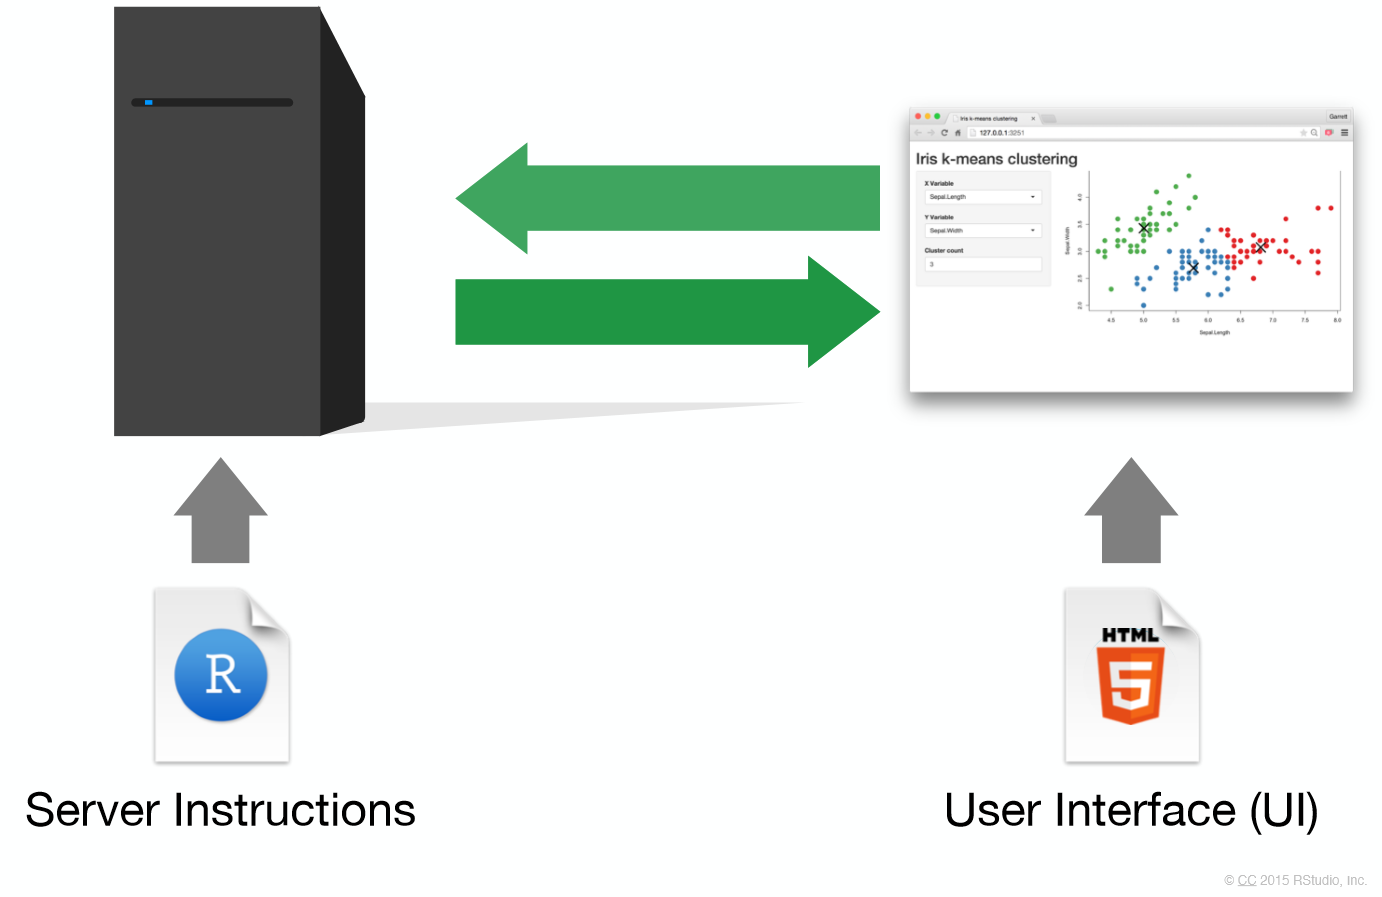
\includegraphics{img/server_R.png}

\section{Ma première application avec
shiny}\label{ma-premiere-application-avec-shiny}

\begin{itemize}
\item
  Initialiser une application est simple avec \textbf{RStudio}, en
  créant un nouveau projet
\item
  File \textgreater{} New Project \textgreater{} New Directory
  \textgreater{} Shiny Web Application
\item
  Basée sur deux scripts : ui.R et server.R
\item
  Et utilisant par défaut le sidebar layout
\item
  Commandes utiles :
\item
  lancement de l'application : bouton \textbf{Run app}
\item
  actualisatisation : bouton \textbf{Reload app}
\item
  arrêt : bouton \textbf{Stop}
\end{itemize}

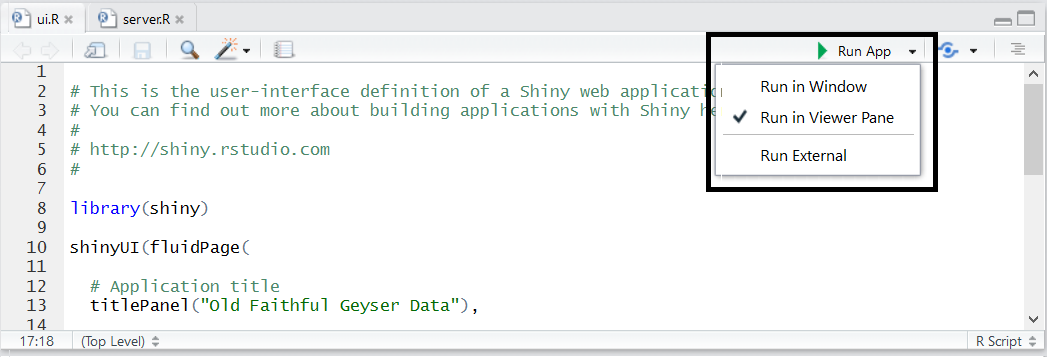
\includegraphics{img/run_app.png}

\begin{itemize}
\tightlist
\item
  \textbf{Run in Window} : Nouvelle fenêtre, utilisant l'environnement
  \textbf{RStudio}
\item
  \textbf{Run in Viewer Pane} : Dans l'onglet \emph{Viewer} de
  \textbf{RStudio}
\item
  \textbf{Run External} : Dans le navigateur web par défaut
\end{itemize}

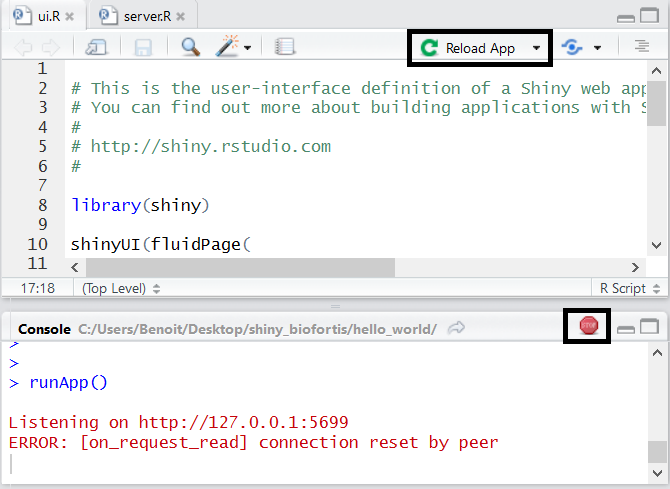
\includegraphics{img/stop.png}

\section{Structure d'une application}\label{structure-dune-application}

\subsection{Un dossier avec un seul
fichier}\label{un-dossier-avec-un-seul-fichier}

\textbf{conventions :}

\begin{itemize}
\tightlist
\item
  enregistré sous le nom \textbf{app.R}
\item
  se terminant par la commande shinyApp()
\item
  pour les \textbf{applications légères}
\end{itemize}

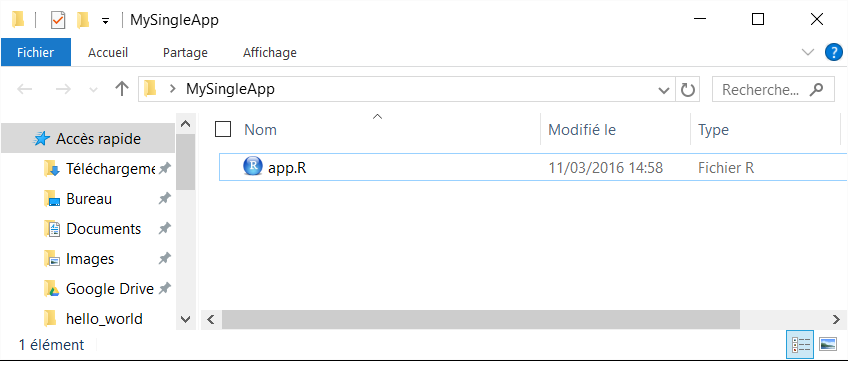
\includegraphics{img/single_app.png}

\begin{Shaded}
\begin{Highlighting}[]
\KeywordTok{library}\NormalTok{(shiny)}
\NormalTok{ui <-}\StringTok{ }\KeywordTok{fluidPage}\NormalTok{(}
  \KeywordTok{sliderInput}\NormalTok{(}\DataTypeTok{inputId =} \StringTok{"num"}\NormalTok{, }\DataTypeTok{label =} \StringTok{"Choose a number"}\NormalTok{, }
              \DataTypeTok{value =} \DecValTok{25}\NormalTok{, }\DataTypeTok{min =} \DecValTok{1}\NormalTok{, }\DataTypeTok{max =} \DecValTok{100}\NormalTok{),  }
  \KeywordTok{plotOutput}\NormalTok{(}\StringTok{"hist"}\NormalTok{)}
\NormalTok{)}
\NormalTok{server <-}\StringTok{ }\ControlFlowTok{function}\NormalTok{(input, output) \{  }
\NormalTok{  output}\OperatorTok{$}\NormalTok{hist <-}\StringTok{ }\KeywordTok{renderPlot}\NormalTok{(\{}
    \KeywordTok{hist}\NormalTok{(}\KeywordTok{rnorm}\NormalTok{(input}\OperatorTok{$}\NormalTok{num))  }
\NormalTok{  \}) }
\NormalTok{\}}
\KeywordTok{shinyApp}\NormalTok{(}\DataTypeTok{ui =}\NormalTok{ ui, }\DataTypeTok{server =}\NormalTok{ server)}
\end{Highlighting}
\end{Shaded}

\subsection{Un dossier avec deux
fichiers}\label{un-dossier-avec-deux-fichiers}

\textbf{conventions :}

\begin{itemize}
\tightlist
\item
  côté interface utilisateur dans le script \textbf{ui.R}
\item
  côté serveur dans le script \textbf{server.R}
\item
  structure à \textbf{priviliégier}
\end{itemize}

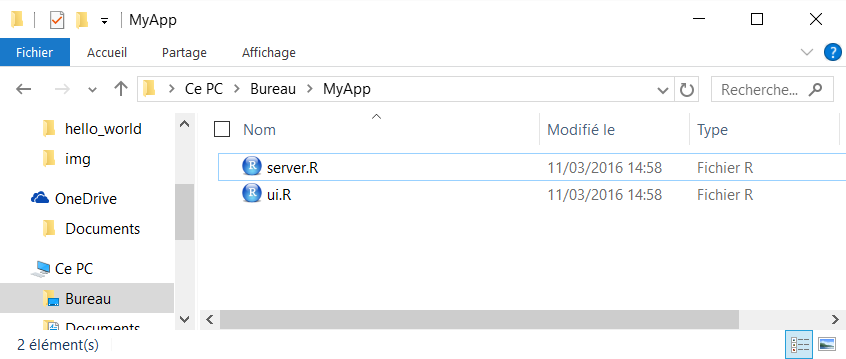
\includegraphics{img/dual_apps.png}

\textbf{ui.R}

\begin{Shaded}
\begin{Highlighting}[]
\KeywordTok{library}\NormalTok{(shiny)}
\KeywordTok{fluidPage}\NormalTok{(}
  \KeywordTok{sliderInput}\NormalTok{(}\DataTypeTok{inputId =} \StringTok{"num"}\NormalTok{, }\DataTypeTok{label =} \StringTok{"Choose a number"}\NormalTok{, }
              \DataTypeTok{value =} \DecValTok{25}\NormalTok{, }\DataTypeTok{min =} \DecValTok{1}\NormalTok{, }\DataTypeTok{max =} \DecValTok{100}\NormalTok{),  }
  \KeywordTok{plotOutput}\NormalTok{(}\StringTok{"hist"}\NormalTok{)}
\NormalTok{)}
\end{Highlighting}
\end{Shaded}

\textbf{server.R}

\begin{Shaded}
\begin{Highlighting}[]
\KeywordTok{library}\NormalTok{(shiny)}
\ControlFlowTok{function}\NormalTok{(input, output) \{  }
\NormalTok{  output}\OperatorTok{$}\NormalTok{hist <-}\StringTok{ }\KeywordTok{renderPlot}\NormalTok{(\{}\KeywordTok{hist}\NormalTok{(}\KeywordTok{rnorm}\NormalTok{(input}\OperatorTok{$}\NormalTok{num))\}) }
\NormalTok{\}}
\end{Highlighting}
\end{Shaded}

\subsection{Données/fichiers
complémentaires}\label{donneesfichiers-complementaires}

\begin{itemize}
\tightlist
\item
  le code \textbf{R} tourne au niveau des scripts \textbf{R}, et peut
  donc accéder de façon relative à tous les objets présents dans le
  dossier de l'application
\item
  l'application web, comme de convention, accède à tous les éléments
  présents dans le dossier \texttt{www} (css, images, javascript,
  documentation, \ldots{})
\end{itemize}

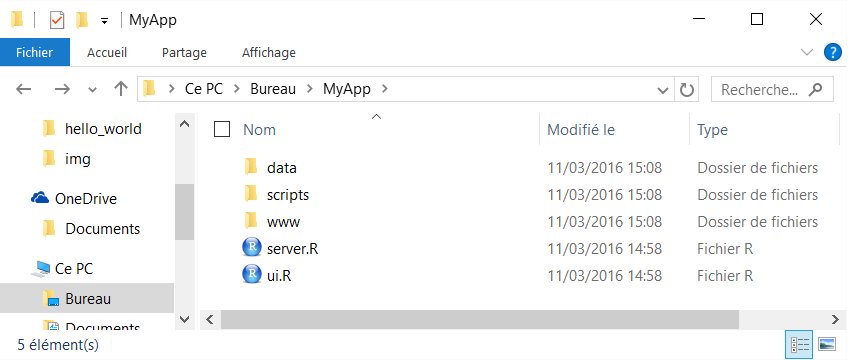
\includegraphics{img/more_apps.png}

\section{Intéractivité et
communication}\label{interactivite-et-communication}

\subsection{Introduction}\label{introduction}

\textbf{ui.R}:

\begin{Shaded}
\begin{Highlighting}[]
\KeywordTok{library}\NormalTok{(shiny)}

\CommentTok{# Define UI for application that draws a histogram}
\KeywordTok{shinyUI}\NormalTok{(}\KeywordTok{fluidPage}\NormalTok{(}
  \CommentTok{# Application title}
  \KeywordTok{titlePanel}\NormalTok{(}\StringTok{"Hello Shiny!"}\NormalTok{),}
  \CommentTok{# Sidebar with a slider input for the number of bins}
  \KeywordTok{sidebarLayout}\NormalTok{(}
    \KeywordTok{sidebarPanel}\NormalTok{(}
      \KeywordTok{sliderInput}\NormalTok{(}\DataTypeTok{inputId =} \StringTok{"bins"}\NormalTok{, }
                  \DataTypeTok{label =} \StringTok{"Number of bins:"}\NormalTok{,}
                  \DataTypeTok{min =} \DecValTok{1}\NormalTok{, }\DataTypeTok{max =} \DecValTok{50}\NormalTok{, }\DataTypeTok{value =} \DecValTok{30}\NormalTok{)}
\NormalTok{    ),}
    \CommentTok{# Show a plot of the generated distribution}
    \KeywordTok{mainPanel}\NormalTok{(}\KeywordTok{plotOutput}\NormalTok{(}\DataTypeTok{outputId =} \StringTok{"distPlot"}\NormalTok{))}
\NormalTok{  )}
\NormalTok{))}
\end{Highlighting}
\end{Shaded}

\textbf{server.R}:

\begin{Shaded}
\begin{Highlighting}[]
\KeywordTok{library}\NormalTok{(shiny)}

\CommentTok{# Define server logic required to draw a histogram}
\KeywordTok{shinyServer}\NormalTok{(}\ControlFlowTok{function}\NormalTok{(input, output) \{}
  \CommentTok{# Expression that generates a histogram. The expression is}
  \CommentTok{# wrapped in a call to renderPlot to indicate that:}
  \CommentTok{#}
  \CommentTok{#  1) It is "reactive" and therefore should be automatically}
  \CommentTok{#     re-executed when inputs change}
  \CommentTok{#  2) Its output type is a plot}
\NormalTok{  output}\OperatorTok{$}\NormalTok{distPlot <-}\StringTok{ }\KeywordTok{renderPlot}\NormalTok{(\{}
\NormalTok{    x    <-}\StringTok{ }\NormalTok{faithful[, }\DecValTok{2}\NormalTok{]  }\CommentTok{# Old Faithful Geyser data}
\NormalTok{    bins <-}\StringTok{ }\KeywordTok{seq}\NormalTok{(}\KeywordTok{min}\NormalTok{(x), }\KeywordTok{max}\NormalTok{(x), }\DataTypeTok{length.out =}\NormalTok{ input}\OperatorTok{$}\NormalTok{bins }\OperatorTok{+}\StringTok{ }\DecValTok{1}\NormalTok{)}
    \CommentTok{# draw the histogram with the specified number of bins}
    \KeywordTok{hist}\NormalTok{(x, }\DataTypeTok{breaks =}\NormalTok{ bins, }\DataTypeTok{col =} \StringTok{'darkgray'}\NormalTok{, }\DataTypeTok{border =} \StringTok{'white'}\NormalTok{)}
\NormalTok{  \})}
\NormalTok{\})}
\end{Highlighting}
\end{Shaded}

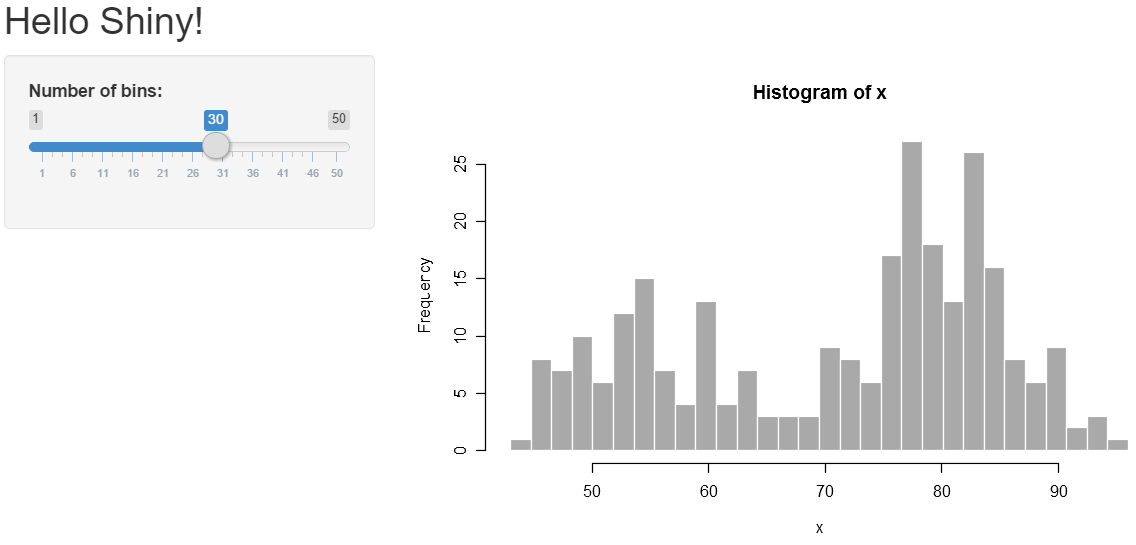
\includegraphics{img/hello_shiny.png}

Avec cette exemple simple, nous comprenons :

\begin{itemize}
\item
  Côté \textbf{ui}, nous définissons un slider numérique avec le code
  ``\texttt{sliderInput(inputId\ =\ "bins",...)}'' et on utilise sa
  valeur côté \textbf{server} avec la notation ``\texttt{input\$bins}''
  : c'est comme cela que le \textbf{ui} créé des variables disponibles
  dans le \textbf{server} !
\item
  Côété \textbf{server}, nous créons un graphique
  ``\texttt{output\$distPlot\ \textless{}-\ renderPlot(\{...\})}'' et
  l'appelons dans le \textbf{ui} avec
  ``\texttt{plotOutput(outputId\ =\ "distPlot")}'', c'est comme cela que
  le \textbf{server} retourne des objet à \textbf{ui} !
\end{itemize}

\subsection{Process}\label{process}

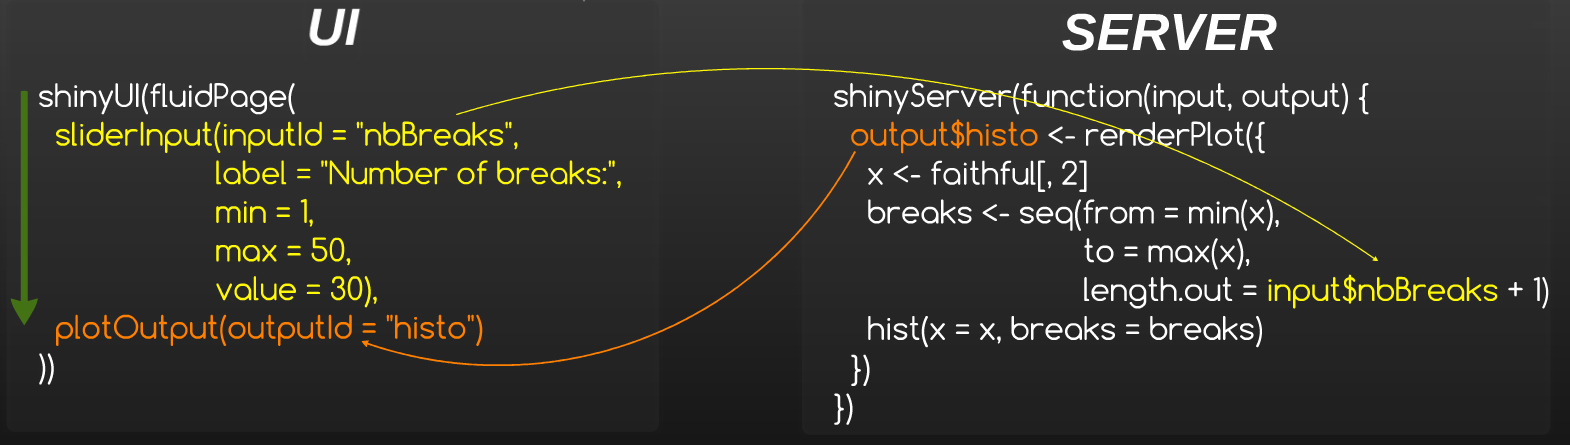
\includegraphics{img/shiny_process.png}

\textbf{Le server et l'ui communiquent uniquement par le biais des
inputs et des outputs}

\textbf{Par défaut, un output est mis-à-jour chaque fois qu'un input en
lien change}

\subsection{Notice}\label{notice}

\textbf{la définition de l'interface utilisateur : UI}

\begin{itemize}
\tightlist
\item
  la déclaration des inputs
\item
  la structure de la page, avec le placement des outputs
\end{itemize}

\textbf{la partie serveur/calculs : SERVER}

\begin{itemize}
\tightlist
\item
  la déclaration et le calcul des outputs
\end{itemize}

\subsection{UI}\label{ui}

\textbf{Deux types d'éléments dans le UI}

\begin{itemize}
\item
  xxInput(inputId = \ldots{}, \ldots{}):
\item
  définit un élément qui permet une action de l'utilisateur
\item
  accessible côté serveur avec son identifiant \textbf{input\$inputID}
\end{itemize}

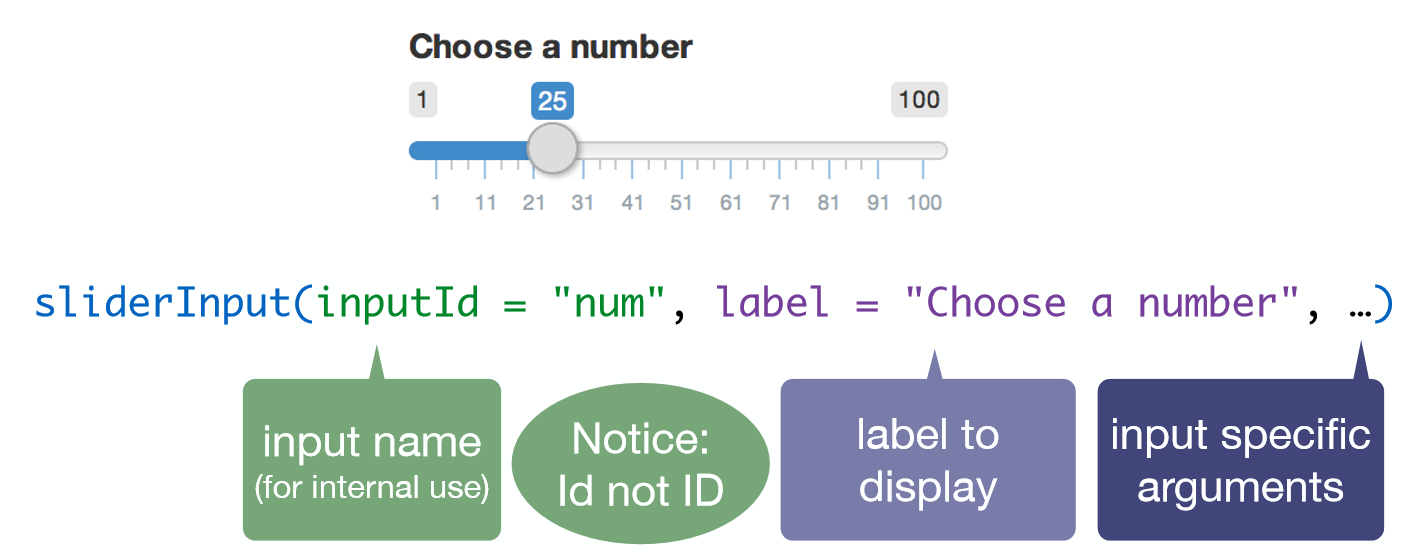
\includegraphics{img/xxInput.png}

\begin{itemize}
\item
  xxOutput(ouputId = \ldots{}):
\item
  fait référence à un output créé et défini côté serveur
\item
  en général : graphiques et tableaux
\end{itemize}

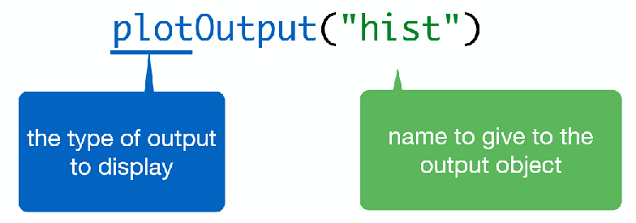
\includegraphics{img/xxOutput.png}

\subsection{Serveur}\label{serveur}

\textbf{Définition des outputs dans le serveur}

\begin{itemize}
\item
  renderXX(\{expr\}):
\item
  calcule et retourne une sortie, dépendante d'inputs, via une
  expression \textbf{R}
\end{itemize}

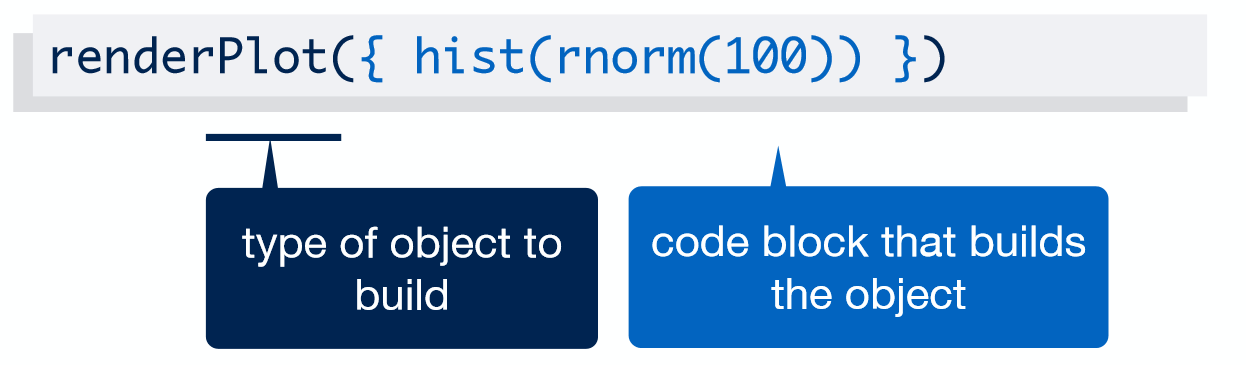
\includegraphics{img/renderXX.png}

\subsection{Retour sur le process}\label{retour-sur-le-process}

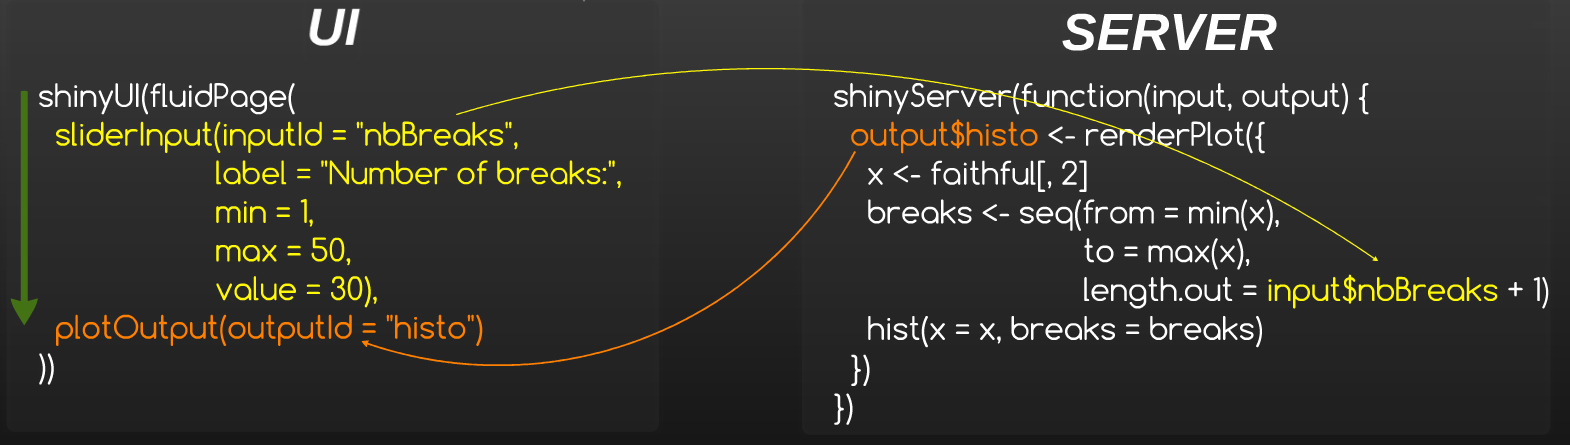
\includegraphics{img/shiny_process.png}

\textbf{C'est plus clair ?}

\subsection{Partage ui \textless{}-\textgreater{}
server}\label{partage-ui---server}

\textbf{Le server et l'ui communiquent uniquement par le biais des
inputs et des outputs}

\begin{itemize}
\item
  Nous pouvons ajouter un script nommé \textbf{global.R} pour partager
  des éléments (variables, packages, \ldots{}) entre la partie
  \textbf{UI} et la partie \textbf{SERVER}
\item
  Tout ce qui est présent dans le \textbf{global.R} est visible à la
  fois dans le \textbf{ui.R} et dans le \textbf{server.R}
\item
  Le script \textbf{global.R} est chargé uniquement une seul fois au
  lancement de l'application
\item
  Dans le cas d'une utilisation avec un \texttt{shiny-server}, les
  objets globaux sont également partagés entre les utilisateurs
\end{itemize}

\section{Les inputs}\label{les-inputs}

\subsection{Vue globale}\label{vue-globale}

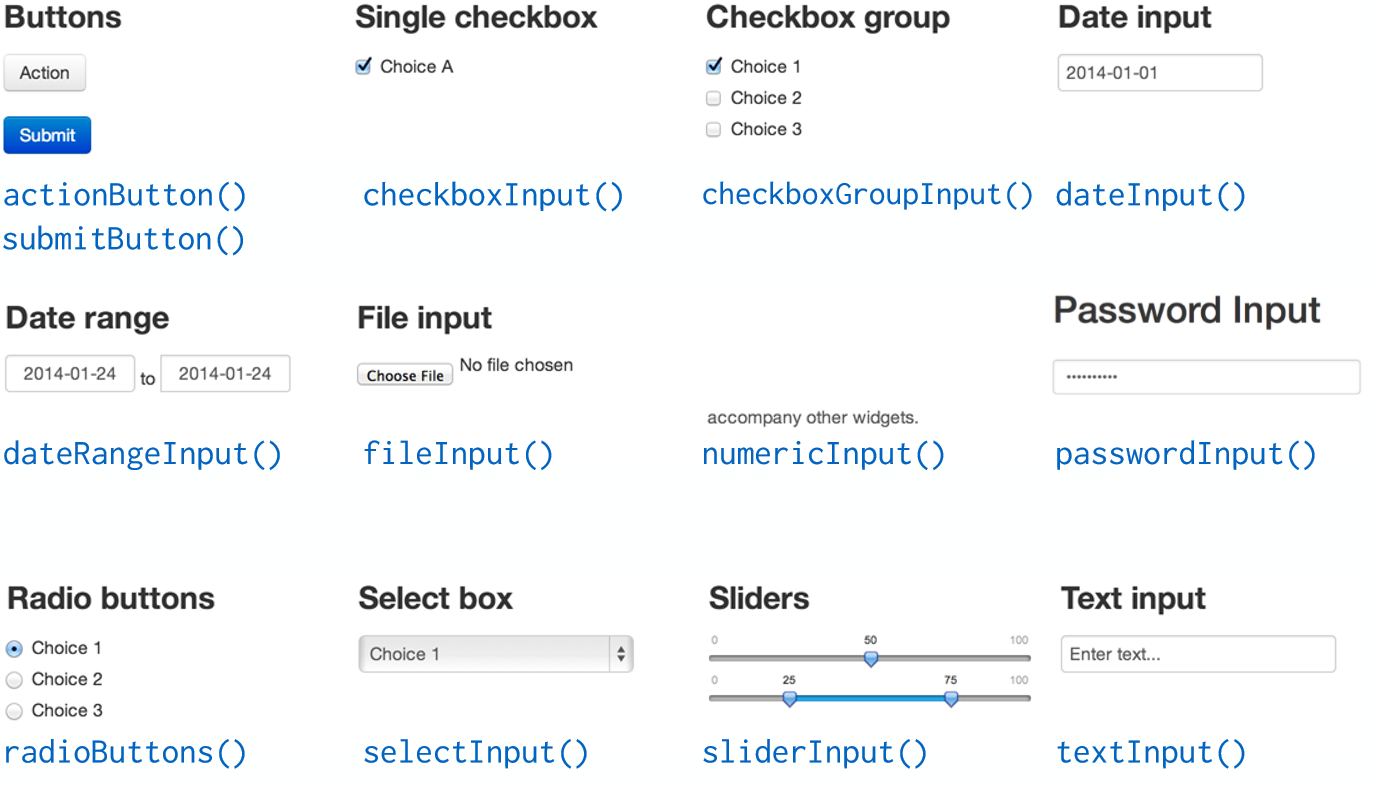
\includegraphics{img/all_input.png}

\subsection{Valeur numérique}\label{valeur-numerique}

\begin{itemize}
\tightlist
\item
  La fonction
\end{itemize}

\begin{Shaded}
\begin{Highlighting}[]
\KeywordTok{numericInput}\NormalTok{(inputId, label, value, }\DataTypeTok{min =} \OtherTok{NA}\NormalTok{, }\DataTypeTok{max =} \OtherTok{NA}\NormalTok{, }\DataTypeTok{step =} \OtherTok{NA}\NormalTok{)}
\end{Highlighting}
\end{Shaded}

\begin{itemize}
\tightlist
\item
  Exemple:
\end{itemize}

\begin{Shaded}
\begin{Highlighting}[]
\KeywordTok{numericInput}\NormalTok{(}\DataTypeTok{inputId =} \StringTok{"idNumeric"}\NormalTok{, }\DataTypeTok{label =} \StringTok{"Please select a number"}\NormalTok{, }
             \DataTypeTok{value =} \DecValTok{0}\NormalTok{, }\DataTypeTok{min =} \DecValTok{0}\NormalTok{, }\DataTypeTok{max =} \DecValTok{100}\NormalTok{, }\DataTypeTok{step =} \DecValTok{10}\NormalTok{)}

\CommentTok{# For the server input$idNumeric will be of class "numeric"}
\CommentTok{# ("integer" when the parameter step is an integer value)}
\end{Highlighting}
\end{Shaded}

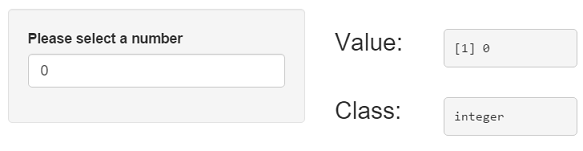
\includegraphics{img/numeric.png}

\subsection{Chaîne de caractères}\label{chaine-de-caracteres}

\begin{itemize}
\tightlist
\item
  La fonction
\end{itemize}

\begin{Shaded}
\begin{Highlighting}[]
\KeywordTok{textInput}\NormalTok{(inputId, label, }\DataTypeTok{value =} \StringTok{""}\NormalTok{)}
\end{Highlighting}
\end{Shaded}

\begin{itemize}
\tightlist
\item
  Exemple:
\end{itemize}

\begin{Shaded}
\begin{Highlighting}[]
\KeywordTok{textInput}\NormalTok{(}\DataTypeTok{inputId =} \StringTok{"idText"}\NormalTok{, }\DataTypeTok{label =} \StringTok{"Enter a text"}\NormalTok{, }\DataTypeTok{value =} \StringTok{""}\NormalTok{)}

\CommentTok{# For the server input$idText will be of class "character" }
\end{Highlighting}
\end{Shaded}

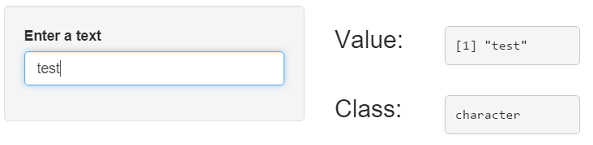
\includegraphics{img/text.png}

\subsection{Liste de sélection}\label{liste-de-selection}

\begin{itemize}
\tightlist
\item
  La fonction
\end{itemize}

\begin{Shaded}
\begin{Highlighting}[]
\KeywordTok{selectInput}\NormalTok{(inputId, label, choices, }\DataTypeTok{selected =} \OtherTok{NULL}\NormalTok{, }\DataTypeTok{multiple =} \OtherTok{FALSE}\NormalTok{,}
            \DataTypeTok{selectize =} \OtherTok{TRUE}\NormalTok{, }\DataTypeTok{width =} \OtherTok{NULL}\NormalTok{, }\DataTypeTok{size =} \OtherTok{NULL}\NormalTok{)}
\end{Highlighting}
\end{Shaded}

\begin{itemize}
\tightlist
\item
  Exemple:
\end{itemize}

\begin{Shaded}
\begin{Highlighting}[]
\KeywordTok{selectInput}\NormalTok{(}\DataTypeTok{inputId =} \StringTok{"idSelect"}\NormalTok{, }\DataTypeTok{label =} \StringTok{"Select among the list: "}\NormalTok{, }\DataTypeTok{selected =} \DecValTok{3}\NormalTok{,}
            \DataTypeTok{choices =} \KeywordTok{c}\NormalTok{(}\StringTok{"First"}\NormalTok{ =}\StringTok{ }\DecValTok{1}\NormalTok{, }\StringTok{"Second"}\NormalTok{ =}\StringTok{ }\DecValTok{2}\NormalTok{, }\StringTok{"Third"}\NormalTok{ =}\StringTok{ }\DecValTok{3}\NormalTok{))}

\CommentTok{# For the server input$idSelect is of class "character"}
\CommentTok{# (vector when the parameter "multiple" is TRUE)}
\end{Highlighting}
\end{Shaded}

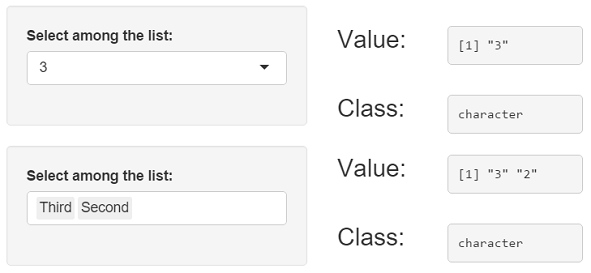
\includegraphics{img/unique_select.png}

\subsection{Checkbox}\label{checkbox}

\begin{itemize}
\tightlist
\item
  La fonction
\end{itemize}

\begin{Shaded}
\begin{Highlighting}[]
\KeywordTok{checkboxInput}\NormalTok{(inputId, label, }\DataTypeTok{value =} \OtherTok{FALSE}\NormalTok{)}
\end{Highlighting}
\end{Shaded}

\begin{itemize}
\tightlist
\item
  Exemple:
\end{itemize}

\begin{Shaded}
\begin{Highlighting}[]
\KeywordTok{checkboxInput}\NormalTok{(}\DataTypeTok{inputId =} \StringTok{"idCheck1"}\NormalTok{, }\DataTypeTok{label =} \StringTok{"Check ?"}\NormalTok{)}

\CommentTok{# For the server input$idCheck1 is of class "logical"}
\end{Highlighting}
\end{Shaded}

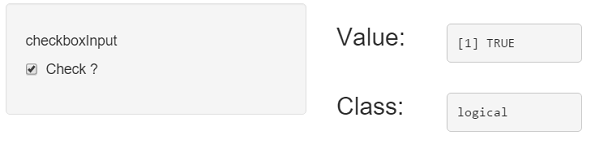
\includegraphics{img/logical.png}

\subsection{Checkboxes multiple}\label{checkboxes-multiple}

\begin{itemize}
\tightlist
\item
  La fonction
\end{itemize}

\begin{Shaded}
\begin{Highlighting}[]
\KeywordTok{checkboxGroupInput}\NormalTok{(inputId, label, choices, }\DataTypeTok{selected =} \OtherTok{NULL}\NormalTok{, }\DataTypeTok{inline =} \OtherTok{FALSE}\NormalTok{)}
\end{Highlighting}
\end{Shaded}

\begin{itemize}
\tightlist
\item
  Exemple:
\end{itemize}

\begin{Shaded}
\begin{Highlighting}[]
\KeywordTok{checkboxGroupInput}\NormalTok{(}\DataTypeTok{inputId =} \StringTok{"idCheckGroup"}\NormalTok{, }\DataTypeTok{label =} \StringTok{"Please select"}\NormalTok{, }\DataTypeTok{selected =} \DecValTok{3}\NormalTok{,}
                   \DataTypeTok{choices =} \KeywordTok{c}\NormalTok{(}\StringTok{"First"}\NormalTok{ =}\StringTok{ }\DecValTok{1}\NormalTok{, }\StringTok{"Second"}\NormalTok{ =}\StringTok{ }\DecValTok{2}\NormalTok{, }\StringTok{"Third"}\NormalTok{ =}\StringTok{ }\DecValTok{3}\NormalTok{))}

\CommentTok{# For the server input$idCheckGroup is a "character" vector}
\end{Highlighting}
\end{Shaded}

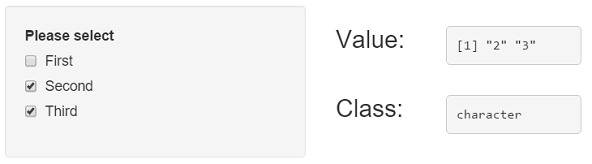
\includegraphics{img/multiple_checkbox.png}

\subsection{Radio boutons}\label{radio-boutons}

\begin{itemize}
\tightlist
\item
  La fonction
\end{itemize}

\begin{Shaded}
\begin{Highlighting}[]
\KeywordTok{radioButtons}\NormalTok{(inputId, label, choices, }\DataTypeTok{selected =} \OtherTok{NULL}\NormalTok{, }\DataTypeTok{inline =} \OtherTok{FALSE}\NormalTok{)}
\end{Highlighting}
\end{Shaded}

\begin{itemize}
\tightlist
\item
  Exemple:
\end{itemize}

\begin{Shaded}
\begin{Highlighting}[]
\KeywordTok{radioButtons}\NormalTok{(}\DataTypeTok{inputId =} \StringTok{"idRadio"}\NormalTok{, }\DataTypeTok{label =} \StringTok{"Select one"}\NormalTok{, }\DataTypeTok{selected =} \DecValTok{3}\NormalTok{,}
             \DataTypeTok{choices =} \KeywordTok{c}\NormalTok{(}\StringTok{"First"}\NormalTok{ =}\StringTok{ }\DecValTok{1}\NormalTok{, }\StringTok{"Second"}\NormalTok{ =}\StringTok{ }\DecValTok{2}\NormalTok{, }\StringTok{"Third"}\NormalTok{ =}\StringTok{ }\DecValTok{3}\NormalTok{))}

\CommentTok{# For the server input$idRadio is a "character"}
\end{Highlighting}
\end{Shaded}

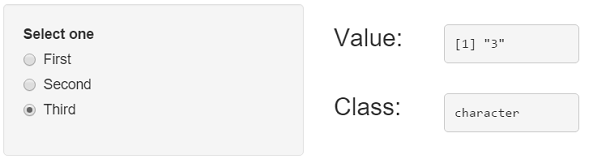
\includegraphics{img/radio.png}

\subsection{Date}\label{date}

\begin{itemize}
\tightlist
\item
  La fonction
\end{itemize}

\begin{Shaded}
\begin{Highlighting}[]
\KeywordTok{dateInput}\NormalTok{(inputId, label, }\DataTypeTok{value =} \OtherTok{NULL}\NormalTok{, }\DataTypeTok{min =} \OtherTok{NULL}\NormalTok{, }\DataTypeTok{max =} \OtherTok{NULL}\NormalTok{, }\DataTypeTok{format =} \StringTok{"yyyy-mm-dd"}\NormalTok{, }
          \DataTypeTok{startview =} \StringTok{"month"}\NormalTok{, }\DataTypeTok{weekstart =} \DecValTok{0}\NormalTok{, }\DataTypeTok{language =} \StringTok{"en"}\NormalTok{)}
\end{Highlighting}
\end{Shaded}

\begin{itemize}
\tightlist
\item
  Exemple:
\end{itemize}

\begin{Shaded}
\begin{Highlighting}[]
\KeywordTok{dateInput}\NormalTok{(}\DataTypeTok{inputId =} \StringTok{"idDate"}\NormalTok{, }\DataTypeTok{label =} \StringTok{"Please enter a date"}\NormalTok{, }\DataTypeTok{value =} \StringTok{"12/08/2015"}\NormalTok{,}
          \DataTypeTok{format =} \StringTok{"dd/mm/yyyy"}\NormalTok{, }\DataTypeTok{startview =} \StringTok{"month"}\NormalTok{, }\DataTypeTok{weekstart =} \DecValTok{0}\NormalTok{, }\DataTypeTok{language =} \StringTok{"fr"}\NormalTok{)}

\CommentTok{# For the server input$idDate is a "Date"}
\end{Highlighting}
\end{Shaded}

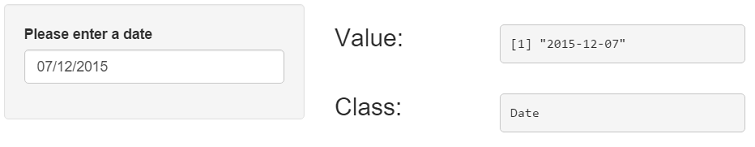
\includegraphics{img/date.png}

\subsection{Période}\label{periode}

\begin{itemize}
\tightlist
\item
  La fonction
\end{itemize}

\begin{Shaded}
\begin{Highlighting}[]
\KeywordTok{dateRangeInput}\NormalTok{(inputId, label, }\DataTypeTok{start =} \OtherTok{NULL}\NormalTok{, }\DataTypeTok{end =} \OtherTok{NULL}\NormalTok{, }\DataTypeTok{min =} \OtherTok{NULL}\NormalTok{, }\DataTypeTok{max =} \OtherTok{NULL}\NormalTok{,}
               \DataTypeTok{format =} \StringTok{"yyyy-mm-dd"}\NormalTok{, }\DataTypeTok{startview =} \StringTok{"month"}\NormalTok{, }\DataTypeTok{weekstart =} \DecValTok{0}\NormalTok{,}
               \DataTypeTok{language =} \StringTok{"en"}\NormalTok{, }\DataTypeTok{separator =} \StringTok{" to "}\NormalTok{)}
\end{Highlighting}
\end{Shaded}

\begin{itemize}
\tightlist
\item
  Exemple:
\end{itemize}

\begin{Shaded}
\begin{Highlighting}[]
\KeywordTok{dateRangeInput}\NormalTok{(}\DataTypeTok{inputId =} \StringTok{"idDateRange"}\NormalTok{, }\DataTypeTok{label =} \StringTok{"Please Select a date range"}\NormalTok{,}
               \DataTypeTok{start =} \StringTok{"2015-01-01"}\NormalTok{, }\DataTypeTok{end =} \StringTok{"2015-08-12"}\NormalTok{, }\DataTypeTok{format =} \StringTok{"yyyy-mm-dd"}\NormalTok{,}
               \DataTypeTok{language =} \StringTok{"en"}\NormalTok{, }\DataTypeTok{separator =} \StringTok{" to "}\NormalTok{)}

\CommentTok{# For the server input$idDateRange is a vector of class "Date" with two elements}
\end{Highlighting}
\end{Shaded}

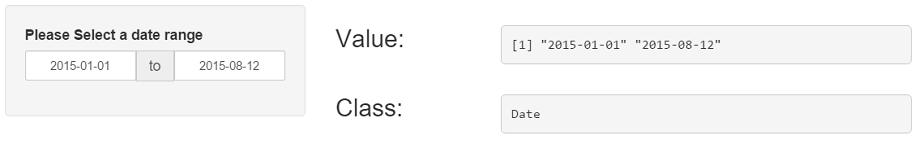
\includegraphics{img/date_range.png}

\subsection{Slider numérique : valeur
unique}\label{slider-numerique-valeur-unique}

\begin{itemize}
\tightlist
\item
  La fonction
\end{itemize}

\begin{Shaded}
\begin{Highlighting}[]
\KeywordTok{sliderInput}\NormalTok{(inputId, label, min, max, value, }\DataTypeTok{step =} \OtherTok{NULL}\NormalTok{, }\DataTypeTok{round =} \OtherTok{FALSE}\NormalTok{,}
            \DataTypeTok{format =} \OtherTok{NULL}\NormalTok{, }\DataTypeTok{locale =} \OtherTok{NULL}\NormalTok{, }\DataTypeTok{ticks =} \OtherTok{TRUE}\NormalTok{, }\DataTypeTok{animate =} \OtherTok{FALSE}\NormalTok{,}
            \DataTypeTok{width =} \OtherTok{NULL}\NormalTok{, }\DataTypeTok{sep =} \StringTok{","}\NormalTok{, }\DataTypeTok{pre =} \OtherTok{NULL}\NormalTok{, }\DataTypeTok{post =} \OtherTok{NULL}\NormalTok{)}
\end{Highlighting}
\end{Shaded}

\begin{itemize}
\tightlist
\item
  Exemple:
\end{itemize}

\begin{Shaded}
\begin{Highlighting}[]
\KeywordTok{sliderInput}\NormalTok{(}\DataTypeTok{inputId =} \StringTok{"idSlider1"}\NormalTok{, }\DataTypeTok{label =} \StringTok{"Select a number"}\NormalTok{, }\DataTypeTok{min =} \DecValTok{0}\NormalTok{, }\DataTypeTok{max =} \DecValTok{10}\NormalTok{, }
            \DataTypeTok{value =} \DecValTok{5}\NormalTok{, }\DataTypeTok{step =} \DecValTok{1}\NormalTok{)}

\CommentTok{# For the server input$idSlider1 is a "numeric"}
\CommentTok{# (integer when the parameter "step" is an integer too)}
\end{Highlighting}
\end{Shaded}

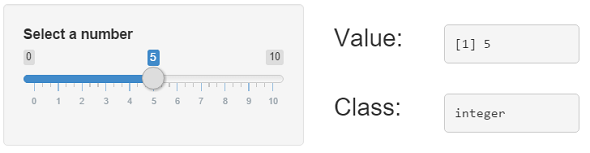
\includegraphics{img/slider.png}

\subsection{Slider numérique : range}\label{slider-numerique-range}

\begin{itemize}
\tightlist
\item
  La fonction
\end{itemize}

\begin{Shaded}
\begin{Highlighting}[]
\KeywordTok{sliderInput}\NormalTok{(inputId, label, min, max, value, }\DataTypeTok{step =} \OtherTok{NULL}\NormalTok{, }\DataTypeTok{round =} \OtherTok{FALSE}\NormalTok{,}
            \DataTypeTok{format =} \OtherTok{NULL}\NormalTok{, }\DataTypeTok{locale =} \OtherTok{NULL}\NormalTok{, }\DataTypeTok{ticks =} \OtherTok{TRUE}\NormalTok{, }\DataTypeTok{animate =} \OtherTok{FALSE}\NormalTok{,}
            \DataTypeTok{width =} \OtherTok{NULL}\NormalTok{, }\DataTypeTok{sep =} \StringTok{","}\NormalTok{, }\DataTypeTok{pre =} \OtherTok{NULL}\NormalTok{, }\DataTypeTok{post =} \OtherTok{NULL}\NormalTok{)}
\end{Highlighting}
\end{Shaded}

\begin{itemize}
\tightlist
\item
  Exemple:
\end{itemize}

\begin{Shaded}
\begin{Highlighting}[]
\KeywordTok{sliderInput}\NormalTok{(}\DataTypeTok{inputId =} \StringTok{"idSlider2"}\NormalTok{, }\DataTypeTok{label =} \StringTok{"Select a number"}\NormalTok{, }\DataTypeTok{min =} \DecValTok{0}\NormalTok{, }\DataTypeTok{max =} \DecValTok{10}\NormalTok{, }
            \DataTypeTok{value =} \KeywordTok{c}\NormalTok{(}\DecValTok{2}\NormalTok{,}\DecValTok{7}\NormalTok{), }\DataTypeTok{step =} \DecValTok{1}\NormalTok{)}

\CommentTok{# For the server input$idSlider2 is a "numeric" vector}
\CommentTok{# (integer when the parameter "step" is an integer too)}
\end{Highlighting}
\end{Shaded}

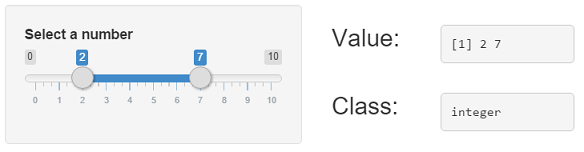
\includegraphics{img/multiple_slider.png}

\subsection{Importer un fichier}\label{importer-un-fichier}

\begin{itemize}
\tightlist
\item
  La fonction
\end{itemize}

\begin{Shaded}
\begin{Highlighting}[]
\KeywordTok{fileInput}\NormalTok{(inputId, label, }\DataTypeTok{multiple =} \OtherTok{FALSE}\NormalTok{, }\DataTypeTok{accept =} \OtherTok{NULL}\NormalTok{)}
\end{Highlighting}
\end{Shaded}

\begin{itemize}
\tightlist
\item
  Exemple:
\end{itemize}

\begin{Shaded}
\begin{Highlighting}[]
\KeywordTok{fileInput}\NormalTok{(}\DataTypeTok{inputId =} \StringTok{"idFile"}\NormalTok{, }\DataTypeTok{label =} \StringTok{"Select a file"}\NormalTok{)}

\CommentTok{# For the server input$idFile is a "data.frame" with four "character" columns}
\CommentTok{# (name, size, type and datapath) and one row}
\end{Highlighting}
\end{Shaded}

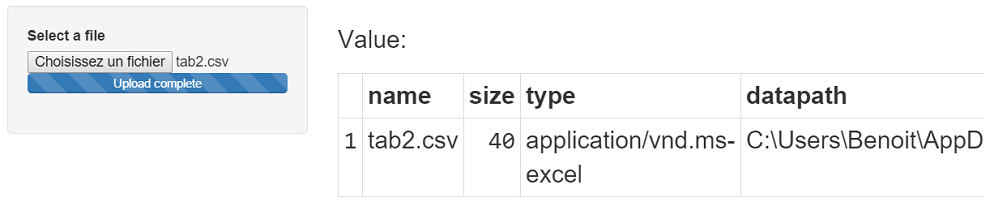
\includegraphics{img/file.png}

\subsection{Action Bouton}\label{action-bouton}

\begin{itemize}
\tightlist
\item
  La fonction
\end{itemize}

\begin{Shaded}
\begin{Highlighting}[]
\KeywordTok{actionButton}\NormalTok{(inputId, label, }\DataTypeTok{icon =} \OtherTok{NULL}\NormalTok{, ...)}
\end{Highlighting}
\end{Shaded}

\begin{itemize}
\tightlist
\item
  Exemple:
\end{itemize}

\begin{Shaded}
\begin{Highlighting}[]
\KeywordTok{actionButton}\NormalTok{(}\DataTypeTok{inputId =} \StringTok{"idActionButton"}\NormalTok{, }\DataTypeTok{label =} \StringTok{"Click !"}\NormalTok{, }
             \DataTypeTok{icon =} \KeywordTok{icon}\NormalTok{(}\StringTok{"hand-spock-o"}\NormalTok{))}

\CommentTok{# For the server input$idActionButton is an "integer"}
\end{Highlighting}
\end{Shaded}

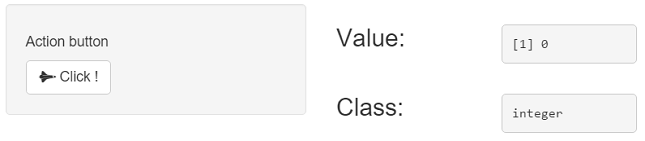
\includegraphics{img/action.png}

\subsection{Aller plus loin : construire son propre
input}\label{aller-plus-loin-construire-son-propre-input}

\textbf{Avec un peu de compétences en HTML/CSS/JavaScript, il est
également possible de construire des inputs personnalisés}

Un tutoriel est disponible :
\url{http://shiny.rstudio.com/articles/building-inputs.html}

Ainsi que deux applications d'exemples :

\begin{itemize}
\item
  \url{http://shiny.rstudio.com/gallery/custom-input-control.html}
\item
  \url{http://shiny.rstudio.com/gallery/custom-input-bindings.html}
\end{itemize}

\section{Outputs}\label{outputs}

\subsection{Vue globale}\label{vue-globale-1}

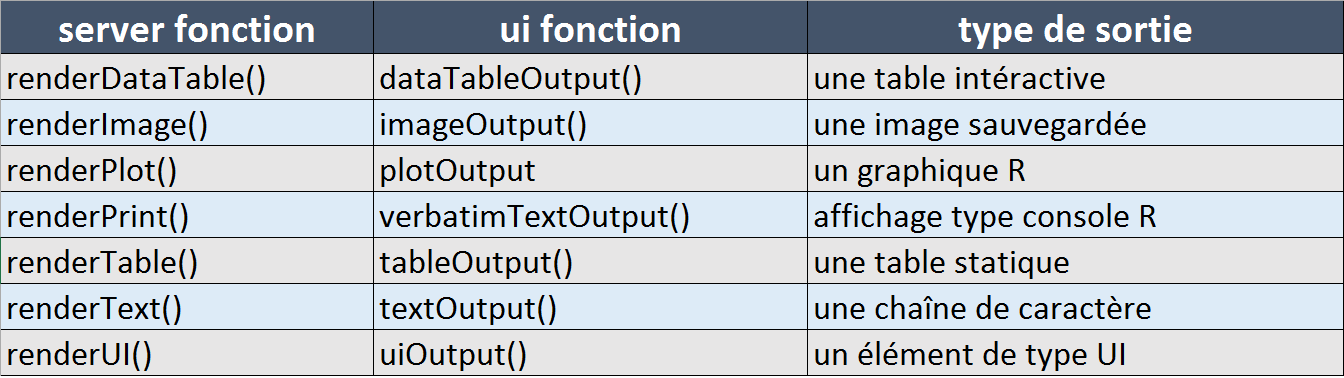
\includegraphics{img/all_output.png}

\subsection{Les bonnes règles de
construction}\label{les-bonnes-regles-de-construction}

\begin{itemize}
\tightlist
\item
  assigner l'output à afficher dans la liste \textbf{output}, avec un
  nom permettant l'identification côté \textbf{UI}
\item
  utiliser une fonction \textbf{renderXX(\{expr\})}
\item
  \textbf{la dernière expression doit correspondre au type d'objet
  retourné}
\item
  accéder aux inputs, et amener la réactivité, en utilisant la liste
  \textbf{input} et l'identifiant : \textbf{input\$inputId}
\end{itemize}

\begin{Shaded}
\begin{Highlighting}[]
\CommentTok{#ui.R}
\KeywordTok{selectInput}\NormalTok{(}\StringTok{"lettre"}\NormalTok{, }\StringTok{"Lettres:"}\NormalTok{, LETTERS[}\DecValTok{1}\OperatorTok{:}\DecValTok{3}\NormalTok{])}
\KeywordTok{verbatimTextOutput}\NormalTok{(}\DataTypeTok{outputId =} \StringTok{"selection"}\NormalTok{)}
\CommentTok{#server.R}
\NormalTok{output}\OperatorTok{$}\NormalTok{selection <-}\StringTok{ }\KeywordTok{renderPrint}\NormalTok{(\{input}\OperatorTok{$}\NormalTok{lettre\})}
\end{Highlighting}
\end{Shaded}

\subsection{Print}\label{print}

\begin{itemize}
\tightlist
\item
  \textbf{ui.r}:
\end{itemize}

\begin{Shaded}
\begin{Highlighting}[]
\KeywordTok{verbatimTextOutput}\NormalTok{(}\DataTypeTok{outputId =} \StringTok{"texte"}\NormalTok{)}
\end{Highlighting}
\end{Shaded}

\begin{itemize}
\tightlist
\item
  \textbf{server.r}:
\end{itemize}

\begin{Shaded}
\begin{Highlighting}[]
\NormalTok{output}\OperatorTok{$}\NormalTok{texte <-}\StringTok{ }\KeywordTok{renderPrint}\NormalTok{(\{}
  \KeywordTok{c}\NormalTok{(}\StringTok{"Hello shiny !"}\NormalTok{)}
\NormalTok{\})}
\end{Highlighting}
\end{Shaded}

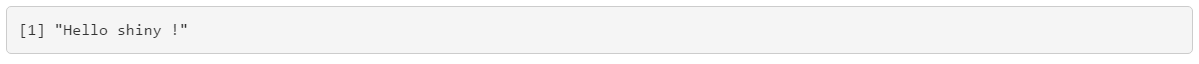
\includegraphics{img/otext.png}

\subsection{Text}\label{text}

\begin{itemize}
\tightlist
\item
  \textbf{ui.r}:
\end{itemize}

\begin{Shaded}
\begin{Highlighting}[]
\KeywordTok{textOutput}\NormalTok{(}\DataTypeTok{outputId =} \StringTok{"texte"}\NormalTok{)}
\end{Highlighting}
\end{Shaded}

\begin{itemize}
\tightlist
\item
  \textbf{server.r}:
\end{itemize}

\begin{Shaded}
\begin{Highlighting}[]
\NormalTok{output}\OperatorTok{$}\NormalTok{texte <-}\StringTok{ }\KeywordTok{renderText}\NormalTok{(\{}
  \KeywordTok{c}\NormalTok{(}\StringTok{"Hello shiny !"}\NormalTok{)}
\NormalTok{\})}
\end{Highlighting}
\end{Shaded}


\includegraphics{img/otext2.png}

\subsubsection{Plot}\label{plot}

\begin{itemize}
\tightlist
\item
  \textbf{ui.r}:
\end{itemize}

\begin{Shaded}
\begin{Highlighting}[]
\KeywordTok{plotOutput}\NormalTok{(}\StringTok{"myplot"}\NormalTok{)}
\end{Highlighting}
\end{Shaded}

\begin{itemize}
\tightlist
\item
  \textbf{server.r}:
\end{itemize}

\begin{Shaded}
\begin{Highlighting}[]
\NormalTok{output}\OperatorTok{$}\NormalTok{myplot <-}\StringTok{ }\KeywordTok{renderPlot}\NormalTok{(\{}
  \KeywordTok{hist}\NormalTok{(iris}\OperatorTok{$}\NormalTok{Sepal.Length)}
\NormalTok{\})}
\end{Highlighting}
\end{Shaded}

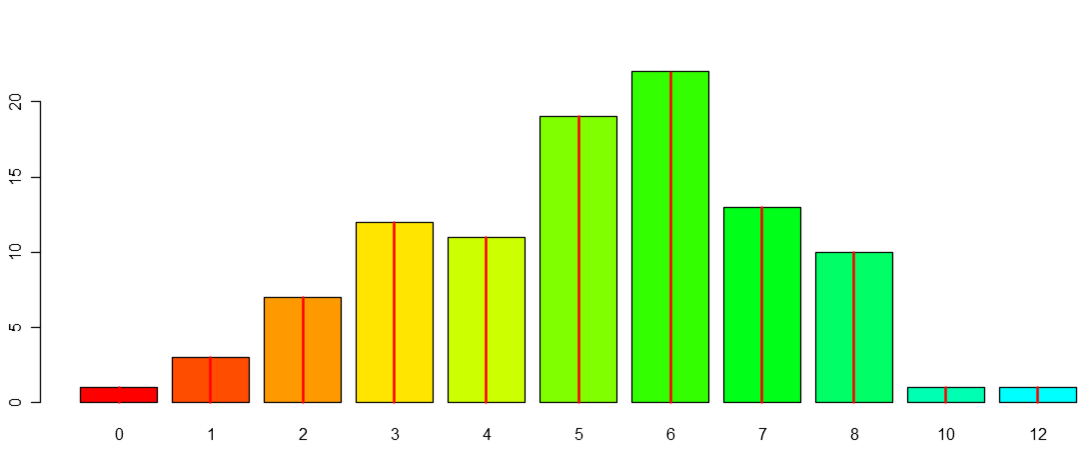
\includegraphics{img/oplot.png}

\subsection{Table}\label{table}

\begin{itemize}
\tightlist
\item
  \textbf{ui.r}:
\end{itemize}

\begin{Shaded}
\begin{Highlighting}[]
\KeywordTok{tableOutput}\NormalTok{(}\DataTypeTok{outputId =} \StringTok{"table"}\NormalTok{)}
\end{Highlighting}
\end{Shaded}

\begin{itemize}
\tightlist
\item
  \textbf{server.r}:
\end{itemize}

\begin{Shaded}
\begin{Highlighting}[]
\NormalTok{output}\OperatorTok{$}\NormalTok{table <-}\StringTok{ }\KeywordTok{renderTable}\NormalTok{(\{iris\})}
\end{Highlighting}
\end{Shaded}

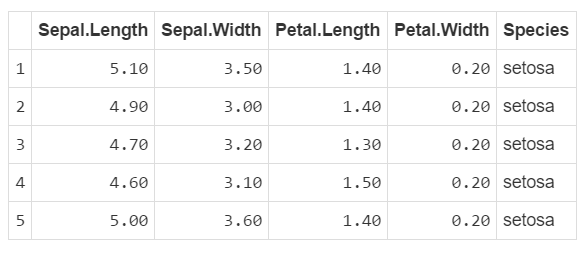
\includegraphics{img/otable.png}

\subsection{DataTable}\label{datatable}

\begin{itemize}
\tightlist
\item
  \textbf{ui.r}:
\end{itemize}

\begin{Shaded}
\begin{Highlighting}[]
\KeywordTok{dataTableOutput}\NormalTok{(}\DataTypeTok{outputId =} \StringTok{"dataTable"}\NormalTok{)}
\end{Highlighting}
\end{Shaded}

\begin{itemize}
\tightlist
\item
  \textbf{server.r}:
\end{itemize}

\begin{Shaded}
\begin{Highlighting}[]
\NormalTok{output}\OperatorTok{$}\NormalTok{dataTable <-}\StringTok{ }\KeywordTok{renderDataTable}\NormalTok{(\{}
\NormalTok{  iris}
\NormalTok{\})}
\end{Highlighting}
\end{Shaded}

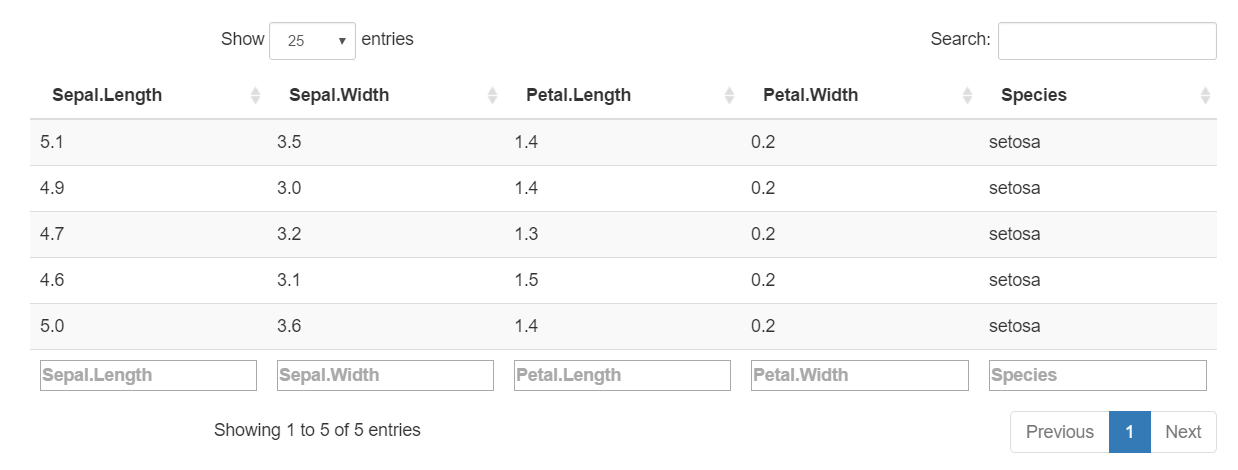
\includegraphics{img/odatable.png}

\subsection{Définir des élements de l'UI côté SERVER \textbar{}
Définition}\label{definir-des-elements-de-lui-cote-server-definition}

\textbf{Dans certains cas, nous souhaitons définir des inputs ou des
structures côté server}

Cela est possible avec les fonctions \texttt{uiOutput} et
\texttt{renderUI}

\subsection{Définir des élements de l'UI côté SERVER \textbar{} Exemple
simple}\label{definir-des-elements-de-lui-cote-server-exemple-simple}

\begin{itemize}
\tightlist
\item
  \textbf{ui.r}:
\end{itemize}

\begin{Shaded}
\begin{Highlighting}[]
\KeywordTok{uiOutput}\NormalTok{(}\DataTypeTok{outputId =} \StringTok{"columns"}\NormalTok{)}
\end{Highlighting}
\end{Shaded}

\begin{itemize}
\tightlist
\item
  \textbf{server.r}:
\end{itemize}

\begin{Shaded}
\begin{Highlighting}[]
\NormalTok{output}\OperatorTok{$}\NormalTok{columns <-}\StringTok{ }\KeywordTok{renderUI}\NormalTok{(\{}
  \KeywordTok{selectInput}\NormalTok{(}\DataTypeTok{inputId =} \StringTok{"sel_col"}\NormalTok{, }\DataTypeTok{label =} \StringTok{"Column"}\NormalTok{, }\DataTypeTok{choices =} \KeywordTok{colnames}\NormalTok{(data))}
\NormalTok{\})}
\end{Highlighting}
\end{Shaded}

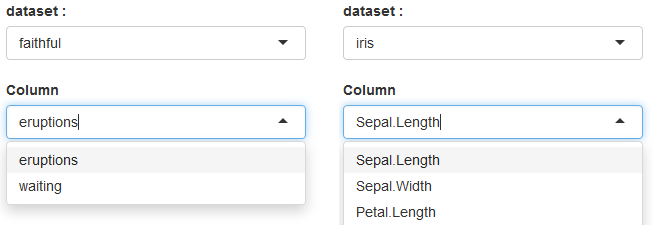
\includegraphics{img/ui_output.png}

\subsection{Définir des élements de l'UI côté SERVER \textbar{} Exemple
plus
complexe}\label{definir-des-elements-de-lui-cote-server-exemple-plus-complexe}

\begin{itemize}
\tightlist
\item
  \textbf{On peut également renvoyer un élément plus complexe de l'UI,
  par exemple :}

  \begin{itemize}
  \tightlist
  \item
    tout en \texttt{layout}
  \item
    ou une \texttt{fluidRow}
  \end{itemize}
\item
  \textbf{ui.r}:
\end{itemize}

\begin{Shaded}
\begin{Highlighting}[]
\KeywordTok{uiOutput}\NormalTok{(}\DataTypeTok{outputId =} \StringTok{"fluidRow_ui"}\NormalTok{)}
\end{Highlighting}
\end{Shaded}

\begin{itemize}
\tightlist
\item
  \textbf{server.r}:
\end{itemize}

\begin{Shaded}
\begin{Highlighting}[]
\NormalTok{output}\OperatorTok{$}\NormalTok{fluidRow_ui <-}\StringTok{ }\KeywordTok{renderUI}\NormalTok{(}
  \KeywordTok{fluidRow}\NormalTok{(}
    \KeywordTok{column}\NormalTok{(}\DataTypeTok{width =} \DecValTok{3}\NormalTok{, }\KeywordTok{h3}\NormalTok{(}\StringTok{"Value:"}\NormalTok{)),}
    \KeywordTok{column}\NormalTok{(}\DataTypeTok{width =} \DecValTok{3}\NormalTok{, }\KeywordTok{h3}\NormalTok{(}\KeywordTok{verbatimTextOutput}\NormalTok{(}\DataTypeTok{outputId =} \StringTok{"slinderIn_value"}\NormalTok{)))}
\NormalTok{  )}
\NormalTok{)}
\end{Highlighting}
\end{Shaded}

\subsection{Aller plus loin : construire son propre
output}\label{aller-plus-loin-construire-son-propre-output}

\textbf{Avec un peu de compétences en HTML/CSS/JavaScript, il est
également possible de construire des outputs personnalisés}

Un tutoriel est disponible :
\url{http://shiny.rstudio.com/articles/building-outputs.html}

On peut donc par exemple ajouter comme output un graphique construit
avec la librairie \href{https://d3js.org/}{d3.js}. Un exemple est
disponible dans le dossier \texttt{shinyApps/build\_output}.

\section{Structurer sa page}\label{structurer-sa-page}

\subsection{sidebarLayout}\label{sidebarlayout}

Le template basique \texttt{sidebarLayout} divise la page en deux
colonnes et doit contenir :

\begin{itemize}
\item
  \texttt{sidebarPanel}, à gauche, en général pour les inputs
\item
  \texttt{mainPanel}, à droite, en général pour les outputs
\end{itemize}

\begin{Shaded}
\begin{Highlighting}[]
\KeywordTok{shinyUI}\NormalTok{(}\KeywordTok{fluidPage}\NormalTok{(}
  \KeywordTok{titlePanel}\NormalTok{(}\StringTok{"Old Faithful Geyser Data"}\NormalTok{), }\CommentTok{# title}
  \KeywordTok{sidebarLayout}\NormalTok{(}
    \KeywordTok{sidebarPanel}\NormalTok{(}\StringTok{"SIDEBAR"}\NormalTok{),}
    \KeywordTok{mainPanel}\NormalTok{(}\StringTok{"MAINPANEL"}\NormalTok{)}
\NormalTok{  )}
\NormalTok{))}
\end{Highlighting}
\end{Shaded}


\includegraphics{img/sidabar.png}

\subsection{wellPanel}\label{wellpanel}

Comme avec le \texttt{sidebarPanel} précédent, on peut griser un
ensemble d'éléments en utilisant un \texttt{wellPanel} :

\begin{Shaded}
\begin{Highlighting}[]
\KeywordTok{shinyUI}\NormalTok{(}\KeywordTok{fluidPage}\NormalTok{(}
  \KeywordTok{titlePanel}\NormalTok{(}\StringTok{"Old Faithful Geyser Data"}\NormalTok{), }\CommentTok{# title}
  \KeywordTok{wellPanel}\NormalTok{(}
    \KeywordTok{sliderInput}\NormalTok{(}\StringTok{"num"}\NormalTok{, }\StringTok{"Choose a number"}\NormalTok{, }\DataTypeTok{value =} \DecValTok{25}\NormalTok{, }\DataTypeTok{min =} \DecValTok{1}\NormalTok{, }\DataTypeTok{max =} \DecValTok{100}\NormalTok{),  }
    \KeywordTok{textInput}\NormalTok{(}\StringTok{"title"}\NormalTok{, }\DataTypeTok{value =} \StringTok{"Histogram"}\NormalTok{, }\DataTypeTok{label =} \StringTok{"Write a title"}\NormalTok{)}
\NormalTok{  ),}
  \KeywordTok{plotOutput}\NormalTok{(}\StringTok{"hist"}\NormalTok{)}
\NormalTok{))}
\end{Highlighting}
\end{Shaded}

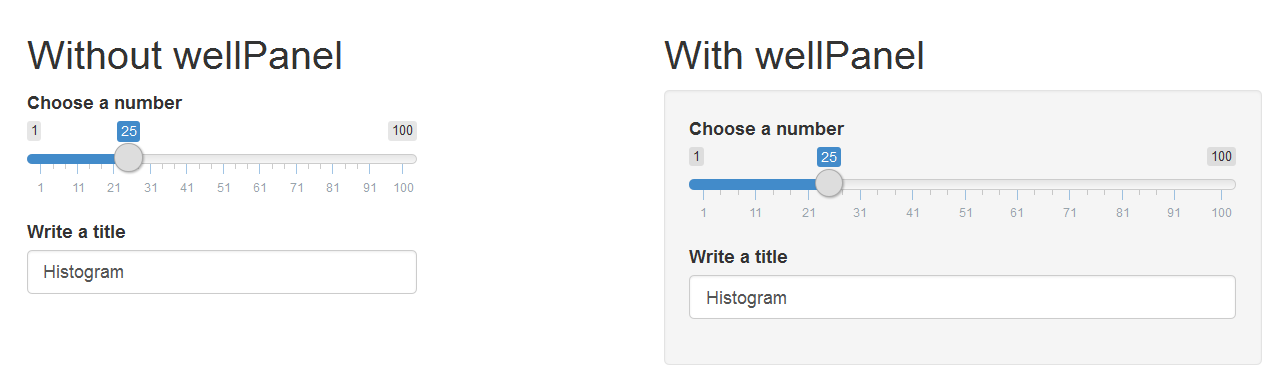
\includegraphics{img/wellPanel.png}

\subsection{navbarPage}\label{navbarpage}

Utiliser une barre de navigation et des onglets avec \texttt{navbarPage}
et \texttt{tabPanel}:

\begin{Shaded}
\begin{Highlighting}[]
\KeywordTok{shinyUI}\NormalTok{(}
  \KeywordTok{navbarPage}\NormalTok{(}
    \DataTypeTok{title =} \StringTok{"My first app"}\NormalTok{,}
    \KeywordTok{tabPanel}\NormalTok{(}\DataTypeTok{title =} \StringTok{"Summary"}\NormalTok{,}
             \StringTok{"Here is the summary"}\NormalTok{),}
    \KeywordTok{tabPanel}\NormalTok{(}\DataTypeTok{title =} \StringTok{"Plot"}\NormalTok{,}
             \StringTok{"some charts"}\NormalTok{),}
    \KeywordTok{tabPanel}\NormalTok{(}\DataTypeTok{title =} \StringTok{"Table"}\NormalTok{,}
             \StringTok{"some tables"}\NormalTok{)}
\NormalTok{  )}
\NormalTok{)}
\end{Highlighting}
\end{Shaded}

Nous pouvons rajouter un second niveau de navigation avec un
\texttt{navbarMenu} :

\begin{Shaded}
\begin{Highlighting}[]
\KeywordTok{shinyUI}\NormalTok{(}
  \KeywordTok{navbarPage}\NormalTok{(}
    \DataTypeTok{title =} \StringTok{"My first app"}\NormalTok{,}
    \KeywordTok{tabPanel}\NormalTok{(}\DataTypeTok{title =} \StringTok{"Summary"}\NormalTok{,}
             \StringTok{"Here is the summary"}\NormalTok{),}
    \KeywordTok{tabPanel}\NormalTok{(}\DataTypeTok{title =} \StringTok{"Plot"}\NormalTok{,}
             \StringTok{"some charts"}\NormalTok{),}
    \KeywordTok{navbarMenu}\NormalTok{(}\StringTok{"Table"}\NormalTok{,}
               \KeywordTok{tabPanel}\NormalTok{(}\StringTok{"Table 1"}\NormalTok{),}
               \KeywordTok{tabPanel}\NormalTok{(}\StringTok{"Table 2"}\NormalTok{)}
\NormalTok{    )}
\NormalTok{  )}
\NormalTok{)}
\end{Highlighting}
\end{Shaded}

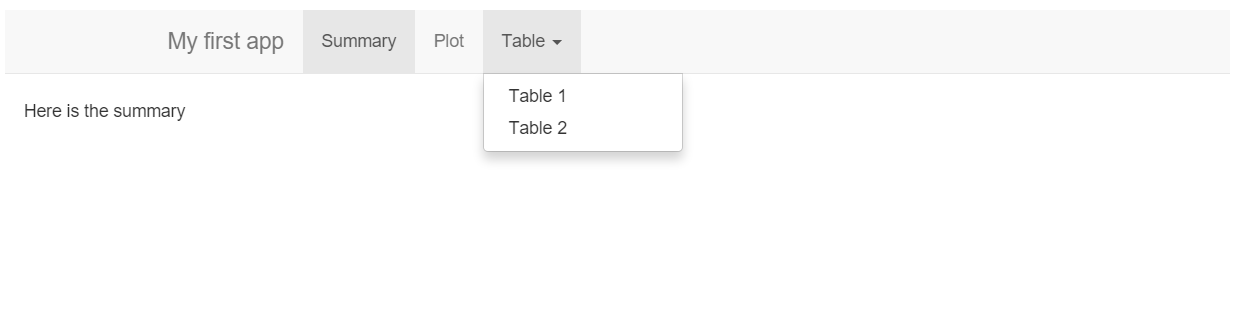
\includegraphics{img/navbar.png}

\subsection{tabsetPanel}\label{tabsetpanel}

Plus généralement, nous pouvons créer des onglets à n'importe quel
endroit en utilisant \texttt{tabsetPanel} \& \texttt{tabPanel}:

\begin{Shaded}
\begin{Highlighting}[]
\KeywordTok{shinyUI}\NormalTok{(}\KeywordTok{fluidPage}\NormalTok{(}
  \KeywordTok{titlePanel}\NormalTok{(}\StringTok{"Old Faithful Geyser Data"}\NormalTok{), }\CommentTok{# title}
  \KeywordTok{sidebarLayout}\NormalTok{(}
    \KeywordTok{sidebarPanel}\NormalTok{(}\StringTok{"SIDEBAR"}\NormalTok{),}
    \KeywordTok{mainPanel}\NormalTok{(}
      \KeywordTok{tabsetPanel}\NormalTok{(}
        \KeywordTok{tabPanel}\NormalTok{(}\StringTok{"Plot"}\NormalTok{, }\KeywordTok{plotOutput}\NormalTok{(}\StringTok{"plot"}\NormalTok{)), }
        \KeywordTok{tabPanel}\NormalTok{(}\StringTok{"Summary"}\NormalTok{, }\KeywordTok{verbatimTextOutput}\NormalTok{(}\StringTok{"summary"}\NormalTok{)), }
        \KeywordTok{tabPanel}\NormalTok{(}\StringTok{"Table"}\NormalTok{, }\KeywordTok{tableOutput}\NormalTok{(}\StringTok{"table"}\NormalTok{))}
\NormalTok{      )}
\NormalTok{    )}
\NormalTok{  )}
\NormalTok{))}
\end{Highlighting}
\end{Shaded}

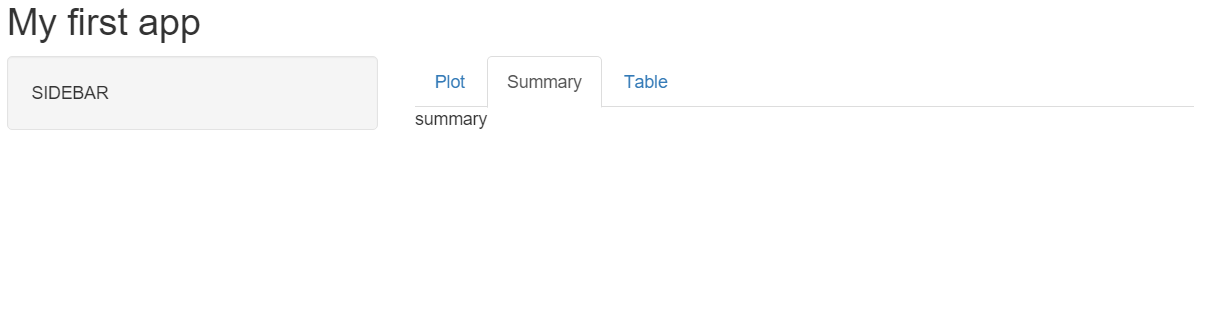
\includegraphics{img/tabpanel.png}

\subsection{navlistPanel}\label{navlistpanel}

Une alternative au \texttt{tabsetPanel}, pour une disposition verticale
plutôt qu'horizontale : \texttt{navlistPanel}

\begin{Shaded}
\begin{Highlighting}[]
\KeywordTok{shinyUI}\NormalTok{(}\KeywordTok{fluidPage}\NormalTok{(}
  \KeywordTok{navlistPanel}\NormalTok{(}
    \KeywordTok{tabPanel}\NormalTok{(}\StringTok{"Plot"}\NormalTok{, }\KeywordTok{plotOutput}\NormalTok{(}\StringTok{"plot"}\NormalTok{)), }
    \KeywordTok{tabPanel}\NormalTok{(}\StringTok{"Summary"}\NormalTok{, }\KeywordTok{verbatimTextOutput}\NormalTok{(}\StringTok{"summary"}\NormalTok{)), }
    \KeywordTok{tabPanel}\NormalTok{(}\StringTok{"Table"}\NormalTok{, }\KeywordTok{tableOutput}\NormalTok{(}\StringTok{"table"}\NormalTok{))}
\NormalTok{  )}
\NormalTok{))}
\end{Highlighting}
\end{Shaded}

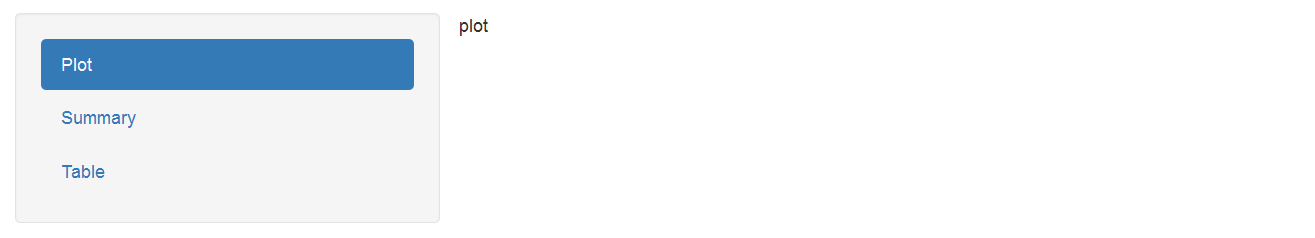
\includegraphics{img/navList.png}

\subsection{Grid Layout}\label{grid-layout}

Créer sa propre organisation avec \texttt{fluidRow()} et
\texttt{column()}

\begin{itemize}
\tightlist
\item
  chaque ligne peut être divisée en 12 colonnes
\item
  le dimensionnement final de la page est automatique en fonction des
  éléments dans les lignes / colonnes
\end{itemize}

\begin{Shaded}
\begin{Highlighting}[]
\KeywordTok{tabPanel}\NormalTok{(}\DataTypeTok{title =} \StringTok{"Summary"}\NormalTok{,}
         \CommentTok{# A fluid row can contain from 0 to 12 columns}
         \KeywordTok{fluidRow}\NormalTok{(}
           \CommentTok{# A column is defined necessarily}
           \CommentTok{# with its argument "width"}
           \KeywordTok{column}\NormalTok{(}\DataTypeTok{width =} \DecValTok{4}\NormalTok{, }\StringTok{"column 1"}\NormalTok{),}
           \KeywordTok{column}\NormalTok{(}\DataTypeTok{width =} \DecValTok{4}\NormalTok{, }\StringTok{"column 2"}\NormalTok{),}
           \KeywordTok{column}\NormalTok{(}\DataTypeTok{width =} \DecValTok{4}\NormalTok{, }\StringTok{"column 3"}\NormalTok{),}
\NormalTok{         ))}
\end{Highlighting}
\end{Shaded}

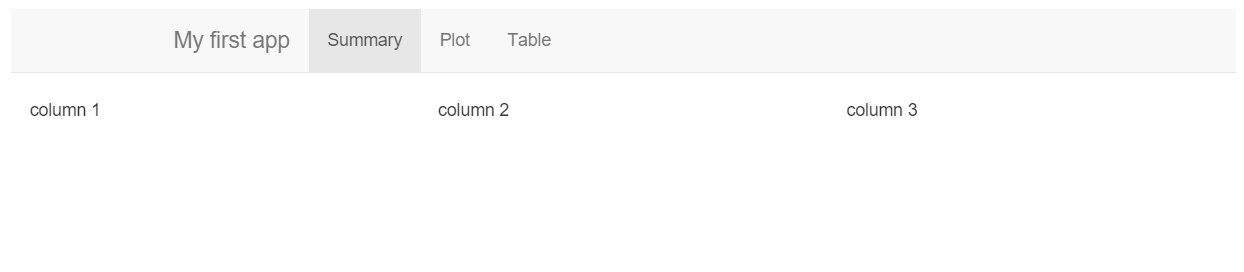
\includegraphics{img/grid.png}

\subsection{shinydashboard}\label{shinydashboard}

Le package
\href{https://rstudio.github.io/shinydashboard/}{shinydashboard} propose
d'autres fonctions pour créer des tableaux de bords :

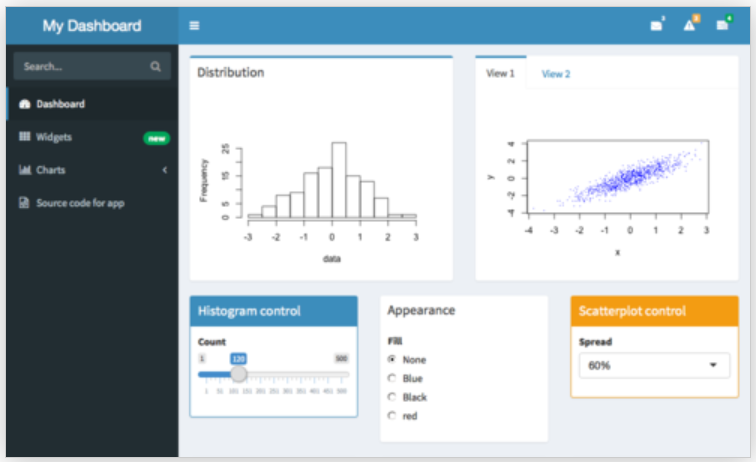
\includegraphics{img/dash.png}

\url{https://rstudio.github.io/shinydashboard/}

\subsection{Combiner les structures}\label{combiner-les-structures}

Toutes les structures peuvent s'utiliser en même temps !

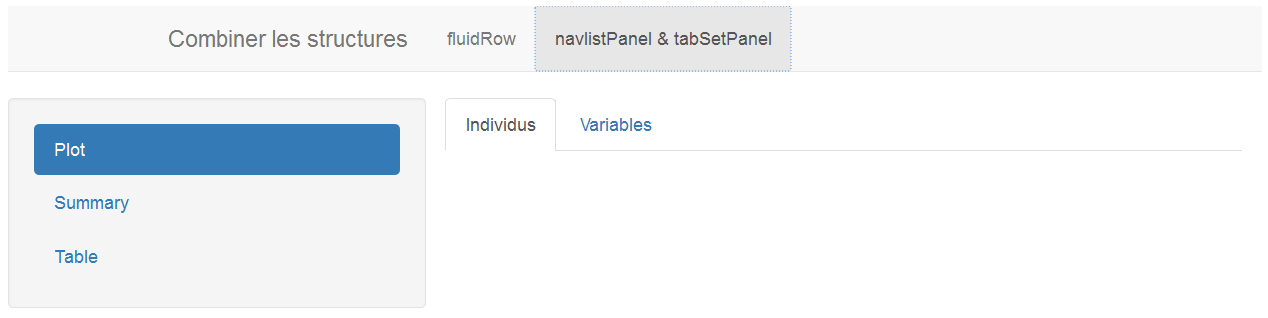
\includegraphics{img/struct.png}

\section{Graphiques intéractifs}\label{graphiques-interactifs}

Avec notamment l'arrivée du package
\href{http://www.htmlwidgets.org/}{htmlwidgets}, de plus en plus de
fonctionnalités de librairies javascript sont accessibles sous
\textbf{R} :

\begin{itemize}
\tightlist
\item
  \href{http://rstudio.github.io/dygraphs/}{dygraphs (time series)}
\item
  \href{http://rstudio.github.io/DT/}{DT (interactive tables)}
\item
  \href{http://rstudio.github.io/leaflet/}{Leafet (maps)}
\item
  \href{https://github.com/rstudio/d3heatmap}{d3heatmap}
\item
  \href{http://bwlewis.github.io/rthreejs}{threejs (3d scatter \&
  globe)}
\item
  \href{http://datastorm-open.github.io/introduction_ramcharts/}{rAmCharts}
\item
  \href{http://datastorm-open.github.io/visNetwork}{visNetwork}
\item
  \ldots{}
\end{itemize}

Plus généralement, jeter un oeil sur la
\href{http://gallery.htmlwidgets.org/}{gallerie suivante!}

\subsection{Utilisation dans shiny}\label{utilisation-dans-shiny}

Tous ces packages sont utilisables simplement dans \textbf{shiny}. En
effet, ils contiennent les deux fonctions nécessaires :

\begin{itemize}
\tightlist
\item
  \textbf{renderXX}
\item
  \textbf{xxOutput}
\end{itemize}

Par exemple avec le package
\href{http://rstudio.github.io/dygraphs/}{dygraphs} :

\begin{Shaded}
\begin{Highlighting}[]
\CommentTok{# Server}
\NormalTok{output}\OperatorTok{$}\NormalTok{dygraph <-}\StringTok{ }\KeywordTok{renderDygraph}\NormalTok{(\{}
  \KeywordTok{dygraph}\NormalTok{(}\KeywordTok{predicted}\NormalTok{(), }\DataTypeTok{main =} \StringTok{"Predicted Deaths/Month"}\NormalTok{)}
\NormalTok{\})}
\CommentTok{# Ui}
\KeywordTok{dygraphOutput}\NormalTok{(}\StringTok{"dygraph"}\NormalTok{)}
\end{Highlighting}
\end{Shaded}

Ces packages arrivent souvent avec des méthodes permettant d'intéragir
avec le graphique, en créant des inputs dans \textbf{shiny} afin de
déclencher des actions . Par exemple :

\begin{itemize}
\tightlist
\item
  \textbf{DT} : création de \emph{input\$tableId\_rows\_selected}, nous
  informant sur la/les lignes sélectionnée(s)
\item
  \textbf{Leaflet} : valeurs du zoom, des clicks, de la
  latitude/longitude, \ldots{}
\item
  \textbf{visNetwork} : noeuds / groupes sélectionnés, \ldots{}
\end{itemize}

Ces points sont (en général) expliqués sur les pages web des différents
packages\ldots{}

De plus, il est également possible d'utiliser de nombreux événements
javascripts, et de crééer des nouvelles intéractions avec \textbf{shiny}
en utilisant \emph{Shiny.onInputChange} :

\begin{Shaded}
\begin{Highlighting}[]
\KeywordTok{visNetwork}\NormalTok{(nodes, edges) }\OperatorTok
\StringTok{      }\KeywordTok{visEvents}\NormalTok{(}\DataTypeTok{hoverNode =} \StringTok{"function(nodes) \{}
\StringTok{        Shiny.onInputChange('current_node_id', nodes);}
\StringTok{      ;\}"}\NormalTok{)}
\end{Highlighting}
\end{Shaded}

\url{https://shiny.rstudio.com/articles/js-send-message.html}

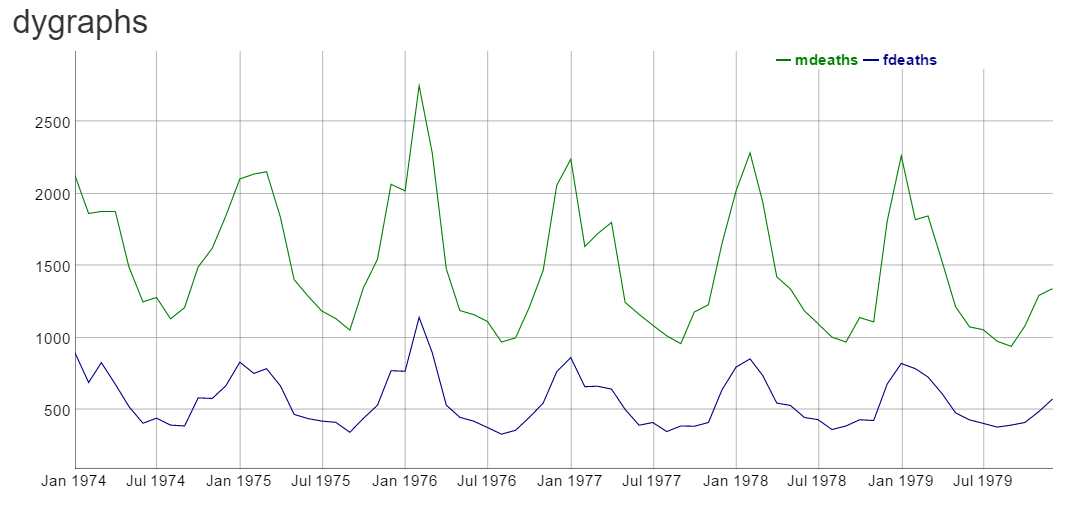
\includegraphics{img/dygraphs.png}

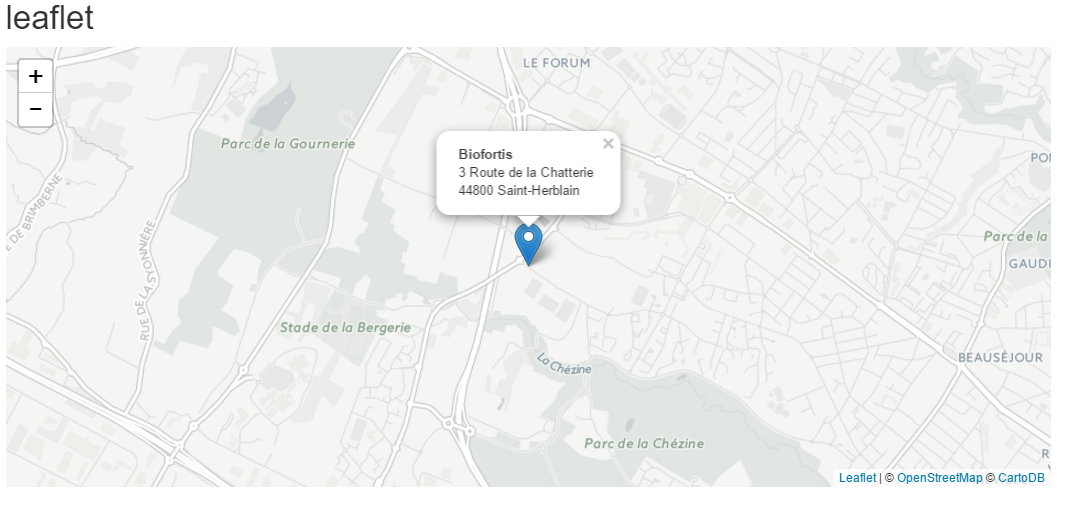
\includegraphics{img/leaflet.png}

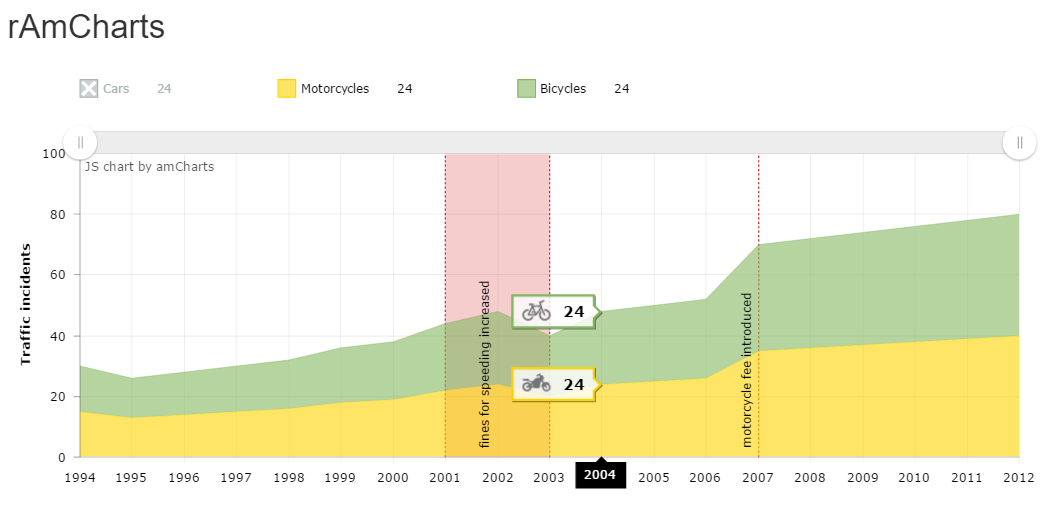
\includegraphics{img/ramcharts.png}

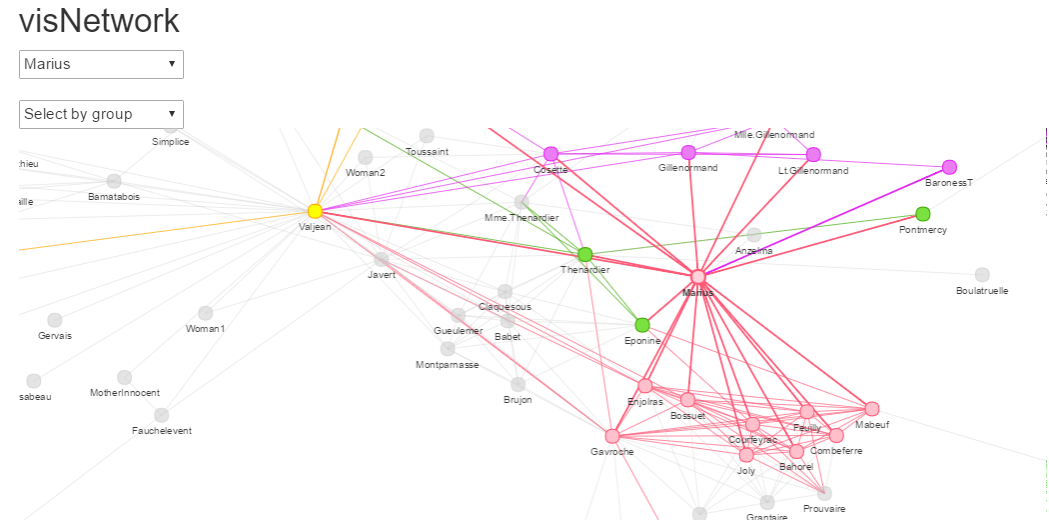
\includegraphics{img/visnetwork.png}

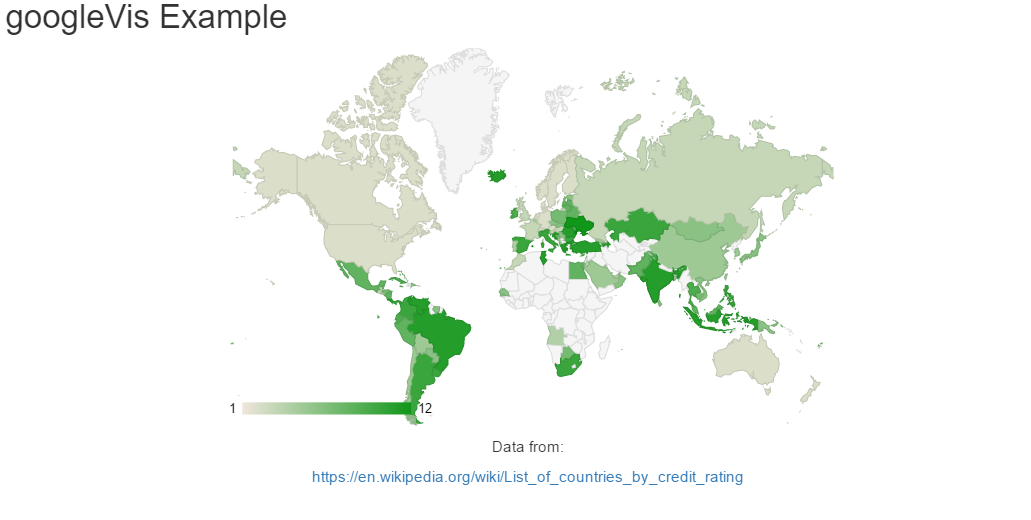
\includegraphics{img/ggvis.png}

\section{Isolation}\label{isolation}

\subsection{Définition}\label{definition}

Par défaut, les outputs et les expressions réactives se mettent à jour
automatiquement quand un des inputs présents dans le code change de
valeur. Dans certains cas, on aimerait pouvoir contrôler un peu cela.

Par exemple, en utilisant un bouton de validation
(\textbf{actionButton}) des inputs pour déclencher le calcul des
sorties.

\begin{itemize}
\item
  un input peut être isolé comme cela \texttt{isolate(input\$id)}
\item
  une expression avec la notation suivante \texttt{isolate(\{expr\})} et
  l'utilisation de \texttt{\{\}}
\end{itemize}

\subsection{Exemple 1}\label{exemple-1}

\begin{itemize}
\tightlist
\item
  \textbf{ui.r}: Trois inputs : \textbf{color} et \textbf{bins} pour
  l'histogramme, et un \textbf{actionButton} :
\end{itemize}

\begin{Shaded}
\begin{Highlighting}[]
\KeywordTok{shinyUI}\NormalTok{(}\KeywordTok{fluidPage}\NormalTok{(}
  \KeywordTok{titlePanel}\NormalTok{(}\StringTok{"Isolation"}\NormalTok{),}
  \KeywordTok{sidebarLayout}\NormalTok{(}
    \KeywordTok{sidebarPanel}\NormalTok{(}
      \KeywordTok{radioButtons}\NormalTok{(}\DataTypeTok{inputId =} \StringTok{"col"}\NormalTok{, }\DataTypeTok{label =} \StringTok{"Choose a color"}\NormalTok{, }\DataTypeTok{inline =} \OtherTok{TRUE}\NormalTok{,}
                   \DataTypeTok{choices =} \KeywordTok{c}\NormalTok{(}\StringTok{"red"}\NormalTok{, }\StringTok{"blue"}\NormalTok{, }\StringTok{"darkgrey"}\NormalTok{)),}
      \KeywordTok{sliderInput}\NormalTok{(}\StringTok{"bins"}\NormalTok{, }\StringTok{"Number of bins:"}\NormalTok{, }\DataTypeTok{min =} \DecValTok{1}\NormalTok{, }\DataTypeTok{max =} \DecValTok{50}\NormalTok{, }\DataTypeTok{value =} \DecValTok{30}\NormalTok{),}
      \KeywordTok{actionButton}\NormalTok{(}\StringTok{"go_graph"}\NormalTok{, }\StringTok{"Update !"}\NormalTok{)}
\NormalTok{    ),}
    \KeywordTok{mainPanel}\NormalTok{(}\KeywordTok{plotOutput}\NormalTok{(}\StringTok{"distPlot"}\NormalTok{))}
\NormalTok{  )}
\NormalTok{))}
\end{Highlighting}
\end{Shaded}

\begin{itemize}
\tightlist
\item
  \textbf{server.r}:
\end{itemize}

On isole tout le code sauf l'\textbf{actionButton} :

\begin{Shaded}
\begin{Highlighting}[]
\KeywordTok{shinyServer}\NormalTok{(}\ControlFlowTok{function}\NormalTok{(input, output) \{}
\NormalTok{  output}\OperatorTok{$}\NormalTok{distPlot <-}\StringTok{ }\KeywordTok{renderPlot}\NormalTok{(\{}
\NormalTok{    input}\OperatorTok{$}\NormalTok{go_graph}
    \KeywordTok{isolate}\NormalTok{(\{}
\NormalTok{      inputColor <-}\StringTok{ }\NormalTok{input}\OperatorTok{$}\NormalTok{color}
\NormalTok{      x <-}\StringTok{ }\NormalTok{faithful[, }\DecValTok{2}\NormalTok{]}
\NormalTok{      bins <-}\StringTok{ }\KeywordTok{seq}\NormalTok{(}\KeywordTok{min}\NormalTok{(x), }\KeywordTok{max}\NormalTok{(x), }\DataTypeTok{length.out =}\NormalTok{ input}\OperatorTok{$}\NormalTok{bins }\OperatorTok{+}\StringTok{ }\DecValTok{1}\NormalTok{)}
      \KeywordTok{hist}\NormalTok{(x, }\DataTypeTok{breaks =}\NormalTok{ bins, }\DataTypeTok{col =}\NormalTok{ inputColor, }\DataTypeTok{border =} \StringTok{'white'}\NormalTok{)}
\NormalTok{    \})}
\NormalTok{  \})}
\NormalTok{\})}
\end{Highlighting}
\end{Shaded}

L'histogramme sera donc mis-à-jour quand l'utilisateur cliquera sur le
bouton.

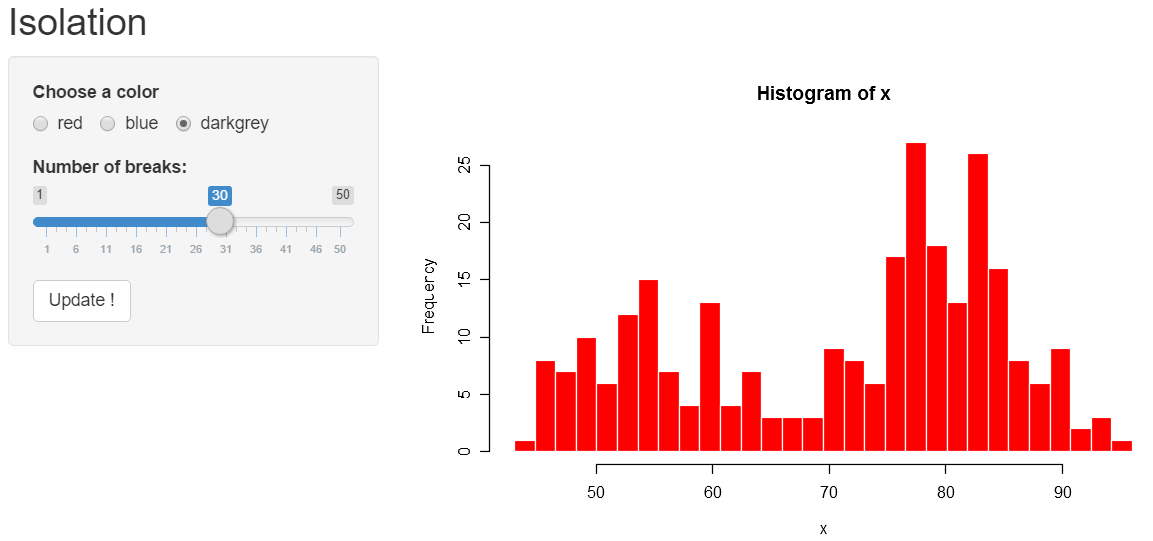
\includegraphics{img/isolation.png}

\subsection{Exemple 2}\label{exemple-2}

\begin{itemize}
\tightlist
\item
  \textbf{server.r}:
\end{itemize}

\begin{Shaded}
\begin{Highlighting}[]
\NormalTok{output}\OperatorTok{$}\NormalTok{distPlot <-}\StringTok{ }\KeywordTok{renderPlot}\NormalTok{(\{}
\NormalTok{  input}\OperatorTok{$}\NormalTok{go_graph}
\NormalTok{  inputColor <-}\StringTok{ }\NormalTok{input}\OperatorTok{$}\NormalTok{color}
  \KeywordTok{isolate}\NormalTok{(\{}
\NormalTok{    x <-}\StringTok{ }\NormalTok{faithful[, }\DecValTok{2}\NormalTok{]}
\NormalTok{    bins <-}\StringTok{ }\KeywordTok{seq}\NormalTok{(}\KeywordTok{min}\NormalTok{(x), }\KeywordTok{max}\NormalTok{(x), }\DataTypeTok{length.out =}\NormalTok{ input}\OperatorTok{$}\NormalTok{bins }\OperatorTok{+}\StringTok{ }\DecValTok{1}\NormalTok{)}
    \KeywordTok{hist}\NormalTok{(x, }\DataTypeTok{breaks =}\NormalTok{ bins, }\DataTypeTok{col =}\NormalTok{ inputColor, }\DataTypeTok{border =} \StringTok{'white'}\NormalTok{)}
\NormalTok{  \})}
\NormalTok{\})}
\end{Highlighting}
\end{Shaded}

Même résultat en isolant seulement le troisième et dernier input
\texttt{input\$bins}

\begin{Shaded}
\begin{Highlighting}[]
\NormalTok{input}\OperatorTok{$}\NormalTok{go_graph}
\NormalTok{x <-}\StringTok{ }\NormalTok{faithful[, }\DecValTok{2}\NormalTok{]}
\NormalTok{bins <-}\StringTok{ }\KeywordTok{seq}\NormalTok{(}\KeywordTok{min}\NormalTok{(x), }\KeywordTok{max}\NormalTok{(x), }\DataTypeTok{length.out =} \KeywordTok{isolate}\NormalTok{(input}\OperatorTok{$}\NormalTok{bins) }\OperatorTok{+}\StringTok{ }\DecValTok{1}\NormalTok{)}
\KeywordTok{hist}\NormalTok{(x, }\DataTypeTok{breaks =}\NormalTok{ bins, }\DataTypeTok{col =}\NormalTok{ input}\OperatorTok{$}\NormalTok{color, }\DataTypeTok{border =} \StringTok{'white'}\NormalTok{)}
\end{Highlighting}
\end{Shaded}

L'histogramme sera donc mis-à-jour quand l'utilisateur cliquera sur le
bouton ou quand la couleur changera.

\section{Expressions réactives}\label{expressions-reactives}

Les expressions réactives sont très utiles quand on souhaite utiliser le
même résultat/objet dans plusieurs outputs, en ne faisant le calcul
qu'une fois.

Il suffit pour cela d'utiliser la fonction \texttt{reactive} dans le
\textbf{server.R}

Par exemple, nous voulons afficher deux graphiques à la suite d'une ACP:

\begin{itemize}
\tightlist
\item
  La projection des individus
\item
  La projection des variables
\end{itemize}

\subsection{Exemple sans une expression
réactive}\label{exemple-sans-une-expression-reactive}

\begin{itemize}
\tightlist
\item
  \textbf{server.R}: le calcul est réalisé deux fois\ldots{}
\end{itemize}

\begin{Shaded}
\begin{Highlighting}[]
\KeywordTok{require}\NormalTok{(FactoMineR) ; }\KeywordTok{data}\NormalTok{(}\StringTok{"decathlon"}\NormalTok{)}

\NormalTok{output}\OperatorTok{$}\NormalTok{graph_pca_ind <-}\StringTok{ }\KeywordTok{renderPlot}\NormalTok{(\{}
\NormalTok{  res_pca <-}\StringTok{ }\KeywordTok{PCA}\NormalTok{(decathlon[ ,input}\OperatorTok{$}\NormalTok{variables], }\DataTypeTok{graph =} \OtherTok{FALSE}\NormalTok{)}
  \KeywordTok{plot.PCA}\NormalTok{(res_pca, }\DataTypeTok{choix =} \StringTok{"ind"}\NormalTok{, }\DataTypeTok{axes =} \KeywordTok{c}\NormalTok{(}\DecValTok{1}\NormalTok{,}\DecValTok{2}\NormalTok{))}
\NormalTok{\})}

\NormalTok{output}\OperatorTok{$}\NormalTok{graph_pca_var <-}\StringTok{ }\KeywordTok{renderPlot}\NormalTok{(\{}
\NormalTok{  res_pca <-}\StringTok{ }\KeywordTok{PCA}\NormalTok{(decathlon[,input}\OperatorTok{$}\NormalTok{variables], }\DataTypeTok{graph =} \OtherTok{FALSE}\NormalTok{)}
  \KeywordTok{plot.PCA}\NormalTok{(res_pca, }\DataTypeTok{choix =} \StringTok{"var"}\NormalTok{, }\DataTypeTok{axes =} \KeywordTok{c}\NormalTok{(}\DecValTok{1}\NormalTok{,}\DecValTok{2}\NormalTok{))}
\NormalTok{\})}
\end{Highlighting}
\end{Shaded}

\subsection{Exemple avec une expression
réactive}\label{exemple-avec-une-expression-reactive}

\begin{itemize}
\tightlist
\item
  \textbf{server.R} : Le calcul est maintenant effectué qu'une seule
  fois !
\end{itemize}

\begin{Shaded}
\begin{Highlighting}[]
\KeywordTok{require}\NormalTok{(FactoMineR) ; }\KeywordTok{data}\NormalTok{(}\StringTok{"decathlon"}\NormalTok{)}

\NormalTok{res_pca <-}\StringTok{ }\KeywordTok{reactive}\NormalTok{(\{}
  \KeywordTok{PCA}\NormalTok{(decathlon[,input}\OperatorTok{$}\NormalTok{variables], }\DataTypeTok{graph =} \OtherTok{FALSE}\NormalTok{)}
\NormalTok{\})}

\NormalTok{output}\OperatorTok{$}\NormalTok{graph_pca_ind <-}\StringTok{ }\KeywordTok{renderPlot}\NormalTok{(\{}
  \KeywordTok{plot.PCA}\NormalTok{(}\KeywordTok{res_pca}\NormalTok{(), }\DataTypeTok{choix =} \StringTok{"ind"}\NormalTok{, }\DataTypeTok{axes =} \KeywordTok{c}\NormalTok{(}\DecValTok{1}\NormalTok{,}\DecValTok{2}\NormalTok{))}
\NormalTok{\})}

\NormalTok{output}\OperatorTok{$}\NormalTok{graph_pca_var <-}\StringTok{ }\KeywordTok{renderPlot}\NormalTok{(\{}
  \KeywordTok{plot.PCA}\NormalTok{(}\KeywordTok{res_pca}\NormalTok{(), }\DataTypeTok{choix =} \StringTok{"var"}\NormalTok{, }\DataTypeTok{axes =} \KeywordTok{c}\NormalTok{(}\DecValTok{1}\NormalTok{,}\DecValTok{2}\NormalTok{))}
\NormalTok{\})}
\end{Highlighting}
\end{Shaded}

\subsection{Note}\label{note}

\begin{itemize}
\item
  Une expression réactive va nous faire gagner du temps et de la mémoire
\item
  \textbf{Utiliser des expressions réactives seulement quand cela dépend
  d'inputs} (pour d'autres variables :
  \url{http://shiny.rstudio.com/articles/scoping.html})
\item
  \textbf{Comme un output} : mis-à-jour chaque fois qu'un input présent
  dans le code change
\item
  \textbf{Comme un input} dans un \emph{renderXX} : l'output est
  mis-à-jour quand l'expression réactive change
\item
  On récupère sa valeur comme un appel à une fonction, avec des ``()''.
\end{itemize}

\subsection{Autres fonctions}\label{autres-fonctions}

Il existe des alternatives à l'utilisation de \texttt{reactive} avec
\texttt{reactiveValues} ou \texttt{reactiveVal}.

\begin{itemize}
\tightlist
\item
  \texttt{reactiveValues} : initialiser une liste d'objets réactifs
\item
  \texttt{reactiveVal} : initialiser un seul objet réactif
\item
  Modification de la valeur des objets avec des \texttt{observe} ou des
  \texttt{observeEvent}
\end{itemize}

\begin{Shaded}
\begin{Highlighting}[]
\KeywordTok{shinyApp}\NormalTok{(}\DataTypeTok{ui =} \KeywordTok{fluidPage}\NormalTok{(}
  \KeywordTok{actionButton}\NormalTok{(}\DataTypeTok{inputId =} \StringTok{"norm"}\NormalTok{, }\DataTypeTok{label =} \StringTok{"Normal"}\NormalTok{),}
  \KeywordTok{actionButton}\NormalTok{(}\DataTypeTok{inputId =} \StringTok{"unif"}\NormalTok{, }\DataTypeTok{label =} \StringTok{"Uniform"}\NormalTok{),}
  \KeywordTok{plotOutput}\NormalTok{(}\StringTok{"hist"}\NormalTok{)}
\NormalTok{), }
\DataTypeTok{server =} \ControlFlowTok{function}\NormalTok{(input, output) \{ }
\NormalTok{  rv <-}\StringTok{ }\KeywordTok{reactiveValues}\NormalTok{(}\DataTypeTok{data =} \KeywordTok{rnorm}\NormalTok{(}\DecValTok{100}\NormalTok{)) }
  \KeywordTok{observeEvent}\NormalTok{(input}\OperatorTok{$}\NormalTok{norm, \{ rv}\OperatorTok{$}\NormalTok{data <-}\StringTok{ }\KeywordTok{rnorm}\NormalTok{(}\DecValTok{100}\NormalTok{) \})   }
  \KeywordTok{observeEvent}\NormalTok{(input}\OperatorTok{$}\NormalTok{unif, \{ rv}\OperatorTok{$}\NormalTok{data <-}\StringTok{ }\KeywordTok{runif}\NormalTok{(}\DecValTok{100}\NormalTok{) \}) }
\NormalTok{  output}\OperatorTok{$}\NormalTok{hist <-}\StringTok{ }\KeywordTok{renderPlot}\NormalTok{(\{ }\KeywordTok{hist}\NormalTok{(rv}\OperatorTok{$}\NormalTok{data) \}) }
\NormalTok{\})}
\end{Highlighting}
\end{Shaded}

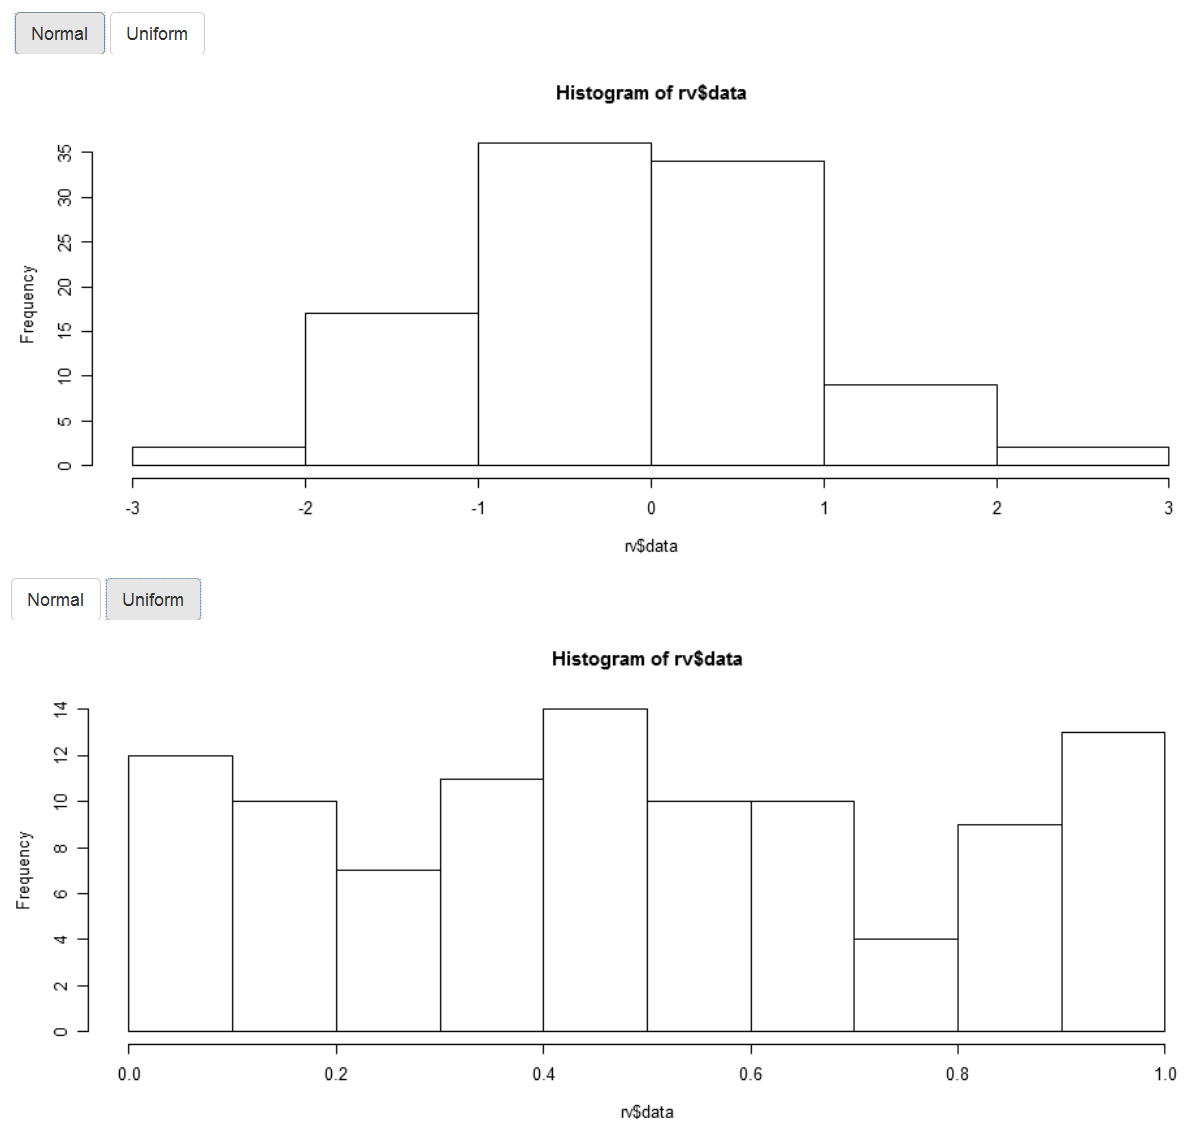
\includegraphics{img/RV.png}

\section{Conditional panels}\label{conditional-panels}

\begin{itemize}
\tightlist
\item
  Il est possible d'afficher conditionnellement ou non certains éléments
  :
\end{itemize}

\begin{verbatim}
conditionalPanel(condition = [...], )
\end{verbatim}

\begin{itemize}
\tightlist
\item
  La condition peut se faire sur des inputs ou des outputs
\item
  Elle doit être rédigée en \textbf{javascript}\ldots{}
\end{itemize}

\begin{verbatim}
conditionalPanel(condition = "input.checkbox == true", [...])
\end{verbatim}

\begin{Shaded}
\begin{Highlighting}[]
\KeywordTok{library}\NormalTok{(shiny)}
\KeywordTok{shinyApp}\NormalTok{(}
  \DataTypeTok{ui =} \KeywordTok{fluidPage}\NormalTok{(}
    \KeywordTok{fluidRow}\NormalTok{(}
      \KeywordTok{column}\NormalTok{(}
        \DataTypeTok{width =} \DecValTok{4}\NormalTok{,}
        \DataTypeTok{align =} \StringTok{"center"}\NormalTok{,}
        \KeywordTok{checkboxInput}\NormalTok{(}\StringTok{"checkbox"}\NormalTok{, }\StringTok{"View other inputs"}\NormalTok{, }\DataTypeTok{value =} \OtherTok{FALSE}\NormalTok{)}
\NormalTok{      ),}
      \KeywordTok{column}\NormalTok{(}
        \DataTypeTok{width =} \DecValTok{8}\NormalTok{,}
        \DataTypeTok{align =} \StringTok{"center"}\NormalTok{,}
        \KeywordTok{conditionalPanel}\NormalTok{(}
          \DataTypeTok{condition =} \StringTok{"input.checkbox == true"}\NormalTok{, }
          \KeywordTok{sliderInput}\NormalTok{(}\StringTok{"slider"}\NormalTok{, }\StringTok{"Select value"}\NormalTok{, }\DataTypeTok{min =} \DecValTok{1}\NormalTok{, }\DataTypeTok{max =} \DecValTok{10}\NormalTok{, }\DataTypeTok{value =} \DecValTok{5}\NormalTok{),}
          \KeywordTok{textInput}\NormalTok{(}\StringTok{"txt"}\NormalTok{, }\StringTok{"Enter text"}\NormalTok{, }\DataTypeTok{value =} \StringTok{""}\NormalTok{)}
\NormalTok{        )}
\NormalTok{      )}
\NormalTok{    )}
\NormalTok{  ),}
  \DataTypeTok{server =} \ControlFlowTok{function}\NormalTok{(input, output) \{\}}
\NormalTok{)}
\end{Highlighting}
\end{Shaded}

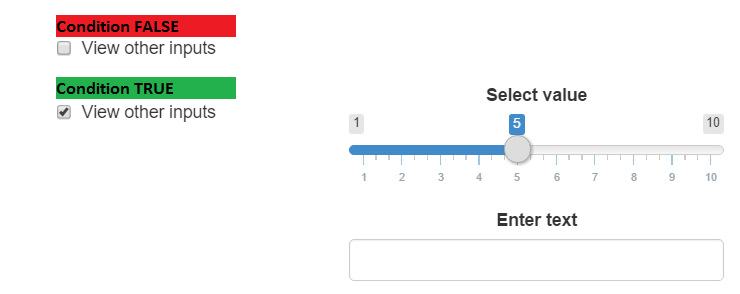
\includegraphics{img/cond1.png}

\section{Observe \& fonctions d'update}\label{observe-fonctions-dupdate}

\subsection{Introduction}\label{introduction-1}

\begin{itemize}
\item
  Il existe une série de fonctions pour mettre à jour les inputs et
  certaines structures
\item
  les fonctions commencent par \texttt{update...}
\item
  On les utilise généralement à l'intérieur d'un
  \texttt{observe(\{expr\})}
\item
  La syntaxe est similaire à celle des fonctions de création
\item
  \textbf{Attention} : il est nécessaire d'ajouter un argument
  \emph{``session''} dans la définition du \textbf{server}
\end{itemize}

\begin{Shaded}
\begin{Highlighting}[]
\KeywordTok{shinyServer}\NormalTok{(}\ControlFlowTok{function}\NormalTok{(input, output, session) \{...\})}
\end{Highlighting}
\end{Shaded}

Sur des inputs :

\begin{itemize}
\tightlist
\item
  \textbf{updateCheckboxGroupInput}
\item
  \textbf{updateCheckboxInput}
\item
  \textbf{updateDateInput Change}
\item
  \textbf{updateDateRangeInput}
\item
  \textbf{updateNumericInput}
\item
  \textbf{updateRadioButtons}
\item
  \textbf{updateSelectInput}
\item
  \textbf{updateSelectizeInput}
\item
  \textbf{updateSliderInput}
\item
  \textbf{updateTextInput}
\end{itemize}

Pour changer dynamiquement l'onglet sélectionné :

\begin{itemize}
\tightlist
\item
  \textbf{updateNavbarPage}, \textbf{updateNavlistPanel},
  \textbf{updateTabsetPanel}
\end{itemize}

\subsection{Exemple sur un input}\label{exemple-sur-un-input}

\begin{Shaded}
\begin{Highlighting}[]
\KeywordTok{shinyUI}\NormalTok{(}\KeywordTok{fluidPage}\NormalTok{(}
  \KeywordTok{titlePanel}\NormalTok{(}\StringTok{"Observe"}\NormalTok{),}
  \KeywordTok{sidebarLayout}\NormalTok{(}
    \KeywordTok{sidebarPanel}\NormalTok{(}
      \KeywordTok{radioButtons}\NormalTok{(}\DataTypeTok{inputId =} \StringTok{"id_dataset"}\NormalTok{, }\DataTypeTok{label =} \StringTok{"Choose a dataset"}\NormalTok{, }\DataTypeTok{inline =} \OtherTok{TRUE}\NormalTok{,}
                   \DataTypeTok{choices =} \KeywordTok{c}\NormalTok{(}\StringTok{"cars"}\NormalTok{, }\StringTok{"iris"}\NormalTok{, }\StringTok{"quakes"}\NormalTok{), }\DataTypeTok{selected =} \StringTok{"cars"}\NormalTok{),}
      \KeywordTok{selectInput}\NormalTok{(}\StringTok{"id_col"}\NormalTok{, }\StringTok{"Choose a column"}\NormalTok{, }\DataTypeTok{choices =} \KeywordTok{colnames}\NormalTok{(cars)),}
      \KeywordTok{textOutput}\NormalTok{(}\DataTypeTok{outputId =} \StringTok{"txt_obs"}\NormalTok{)}
\NormalTok{    ),}
    \KeywordTok{mainPanel}\NormalTok{(}\KeywordTok{fluidRow}\NormalTok{(}
      \KeywordTok{dataTableOutput}\NormalTok{(}\DataTypeTok{outputId =} \StringTok{"dataset_obs"}\NormalTok{)}
\NormalTok{    ))}
\NormalTok{  )}
\NormalTok{))}
\end{Highlighting}
\end{Shaded}

\begin{Shaded}
\begin{Highlighting}[]
\KeywordTok{shinyServer}\NormalTok{(}\ControlFlowTok{function}\NormalTok{(input, output, session) \{}
\NormalTok{  dataset <-}\StringTok{ }\KeywordTok{reactive}\NormalTok{(}\KeywordTok{get}\NormalTok{(input}\OperatorTok{$}\NormalTok{id_dataset, }\StringTok{"package:datasets"}\NormalTok{))}
  
  \KeywordTok{observe}\NormalTok{(\{}
    \KeywordTok{updateSelectInput}\NormalTok{(session, }\DataTypeTok{inputId =} \StringTok{"id_col"}\NormalTok{, }\DataTypeTok{label =} \StringTok{"Choose a column"}\NormalTok{,}
                      \DataTypeTok{choices =} \KeywordTok{colnames}\NormalTok{(}\KeywordTok{dataset}\NormalTok{()))}
\NormalTok{  \})}
  
\NormalTok{  output}\OperatorTok{$}\NormalTok{txt_obs <-}\StringTok{ }\KeywordTok{renderText}\NormalTok{(}\KeywordTok{paste0}\NormalTok{(}\StringTok{"Selected column : "}\NormalTok{, input}\OperatorTok{$}\NormalTok{id_col))}
  
\NormalTok{  output}\OperatorTok{$}\NormalTok{dataset_obs <-}\StringTok{ }\KeywordTok{renderDataTable}\NormalTok{(}
    \KeywordTok{dataset}\NormalTok{(),}
    \DataTypeTok{options =} \KeywordTok{list}\NormalTok{(}\DataTypeTok{pageLength =} \DecValTok{5}\NormalTok{)}
\NormalTok{  )}
\NormalTok{\})}
\end{Highlighting}
\end{Shaded}

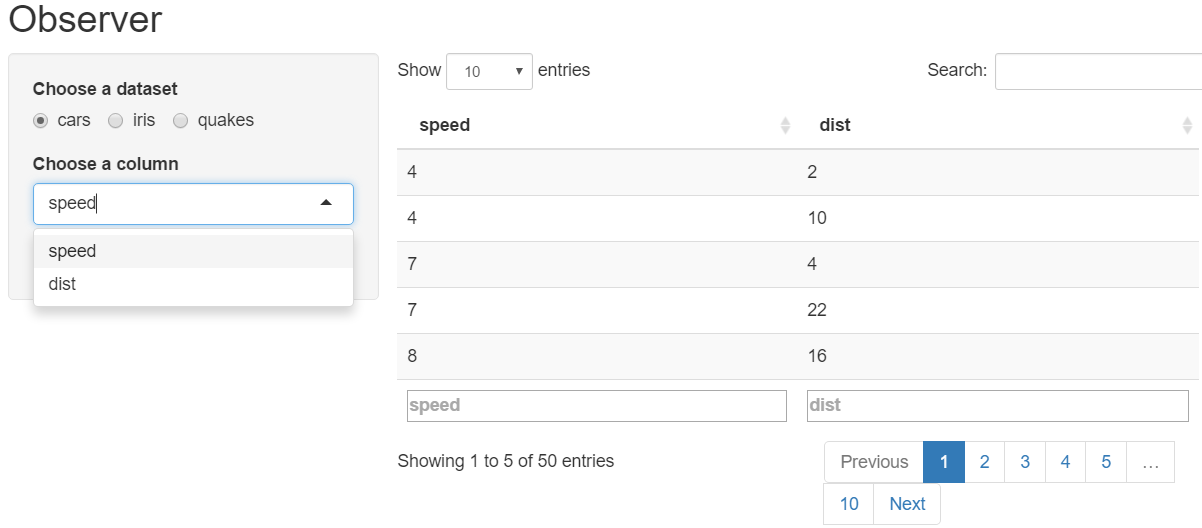
\includegraphics{img/observer1.png}

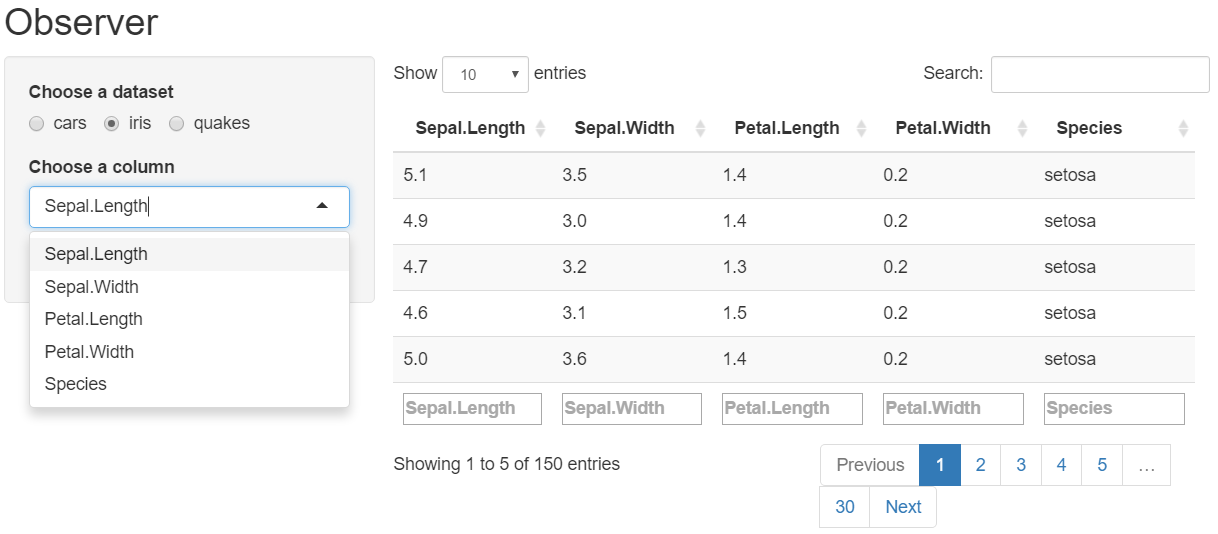
\includegraphics{img/observer2.png}

\subsection{Exemple sur des onglets}\label{exemple-sur-des-onglets}

\textbf{Il faut rajouter un id dans la structure}

\begin{Shaded}
\begin{Highlighting}[]
\KeywordTok{shinyUI}\NormalTok{(}
  \KeywordTok{navbarPage}\NormalTok{(}
    \DataTypeTok{id =} \StringTok{"idnavbar"}\NormalTok{, }\CommentTok{# need an id for oberve & update}
    \DataTypeTok{title =} \StringTok{"A NavBar"}\NormalTok{,}
    \KeywordTok{tabPanel}\NormalTok{(}\DataTypeTok{title =} \StringTok{"Summary"}\NormalTok{,}
             \KeywordTok{actionButton}\NormalTok{(}\StringTok{"goPlot"}\NormalTok{, }\StringTok{"Go to plot !"}\NormalTok{)),}
    \KeywordTok{tabPanel}\NormalTok{(}\DataTypeTok{title =} \StringTok{"Plot"}\NormalTok{,}
             \KeywordTok{actionButton}\NormalTok{(}\StringTok{"goSummary"}\NormalTok{, }\StringTok{"Go to Summary !"}\NormalTok{))}
    
\NormalTok{  )}
\NormalTok{)}
\end{Highlighting}
\end{Shaded}

\begin{Shaded}
\begin{Highlighting}[]
\KeywordTok{shinyServer}\NormalTok{(}\ControlFlowTok{function}\NormalTok{(input, output, session) \{}
  \KeywordTok{observe}\NormalTok{(\{}
\NormalTok{    input}\OperatorTok{$}\NormalTok{goPlot}
    \KeywordTok{updateTabsetPanel}\NormalTok{(session, }\StringTok{"idnavbar"}\NormalTok{, }\DataTypeTok{selected =} \StringTok{"Plot"}\NormalTok{)}
\NormalTok{  \})}
  \KeywordTok{observe}\NormalTok{(\{}
\NormalTok{    input}\OperatorTok{$}\NormalTok{goSummary}
    \KeywordTok{updateTabsetPanel}\NormalTok{(session, }\StringTok{"idnavbar"}\NormalTok{, }\DataTypeTok{selected =} \StringTok{"Summary"}\NormalTok{)}
\NormalTok{  \})}
\NormalTok{\})}
\end{Highlighting}
\end{Shaded}

\subsection{observeEvent}\label{observeevent}

\begin{itemize}
\tightlist
\item
  Une variante de la fonction \texttt{observe} est disponible avec la
  fonction \texttt{observeEvent}
\item
  On définit alors de façon explicite l'espression qui représente
  l'événement \emph{et} l'expression qui sera éxécutée quand l'événement
  se produit
\end{itemize}

\begin{Shaded}
\begin{Highlighting}[]
\CommentTok{# avec un observe}
\KeywordTok{observe}\NormalTok{(\{}
\NormalTok{  input}\OperatorTok{$}\NormalTok{goPlot}
  \KeywordTok{updateTabsetPanel}\NormalTok{(session, }\StringTok{"idnavbar"}\NormalTok{, }\DataTypeTok{selected =} \StringTok{"Plot"}\NormalTok{)}
\NormalTok{\})}

\CommentTok{# idem avec un observeEvent}
\KeywordTok{observeEvent}\NormalTok{(input}\OperatorTok{$}\NormalTok{goSummary, \{}
  \KeywordTok{updateTabsetPanel}\NormalTok{(session, }\StringTok{"idnavbar"}\NormalTok{, }\DataTypeTok{selected =} \StringTok{"Summary"}\NormalTok{)}
\NormalTok{\})}
\end{Highlighting}
\end{Shaded}

\section{HTML / CSS}\label{html-css}

\subsection{Inclure du HTML}\label{inclure-du-html}

De nombreuses de balises \textbf{html} sont disponibles avec les
fonctions \texttt{tags} :

\begin{Shaded}
\begin{Highlighting}[]
\KeywordTok{names}\NormalTok{(shiny}\OperatorTok{::}\NormalTok{tags)}
\end{Highlighting}
\end{Shaded}

\begin{verbatim}
##   [1] "a"           "abbr"        "address"     "area"        "article"    
##   [6] "aside"       "audio"       "b"           "base"        "bdi"        
##  [11] "bdo"         "blockquote"  "body"        "br"          "button"     
##  [16] "canvas"      "caption"     "cite"        "code"        "col"        
##  [21] "colgroup"    "command"     "data"        "datalist"    "dd"         
##  [26] "del"         "details"     "dfn"         "div"         "dl"         
##  [31] "dt"          "em"          "embed"       "eventsource" "fieldset"   
##  [36] "figcaption"  "figure"      "footer"      "form"        "h1"         
##  [41] "h2"          "h3"          "h4"          "h5"          "h6"         
##  [46] "head"        "header"      "hgroup"      "hr"          "html"       
##  [51] "i"           "iframe"      "img"         "input"       "ins"        
##  [56] "kbd"         "keygen"      "label"       "legend"      "li"         
##  [61] "link"        "mark"        "map"         "menu"        "meta"       
##  [66] "meter"       "nav"         "noscript"    "object"      "ol"         
##  [71] "optgroup"    "option"      "output"      "p"           "param"      
##  [76] "pre"         "progress"    "q"           "ruby"        "rp"         
##  [81] "rt"          "s"           "samp"        "script"      "section"    
##  [86] "select"      "small"       "source"      "span"        "strong"     
##  [91] "style"       "sub"         "summary"     "sup"         "table"      
##  [96] "tbody"       "td"          "textarea"    "tfoot"       "th"         
## [101] "thead"       "time"        "title"       "tr"          "track"      
## [106] "u"           "ul"          "var"         "video"       "wbr"
\end{verbatim}

\includegraphics{img/tags.png}

C'est également possible de passer du code \textbf{HTML} directement en
utilisant la fonction du même nom :

\begin{Shaded}
\begin{Highlighting}[]
\KeywordTok{fluidPage}\NormalTok{(}
  \KeywordTok{HTML}\NormalTok{(}\StringTok{"<h1>My Shiny App</h1>"}\NormalTok{) }
\NormalTok{)}
\end{Highlighting}
\end{Shaded}

\subsection{Quelques balises utiles}\label{quelques-balises-utiles}

\begin{itemize}
\tightlist
\item
  \texttt{div(...,\ align\ =\ "center")} : centrer les éléments
\item
  \texttt{br()} : saut de ligne
\item
  \texttt{hr()} : trait horizontal
\item
  \texttt{img(src="img/logo.jpg",\ title="Popup",\ width\ =\ "80\%")} :
  insertion d'une image présente dans \textbf{www/img}
\item
  \texttt{a(href="https://r2018-rennes.sciencesconf.org/",\ target="\_blank",\ "Rencontres\ R")}
  : lien vers un site
\item
  \texttt{a(href\ =\ \textquotesingle{}./doc/guide.pdf\textquotesingle{},\ target="\_blank",\ class\ =\ "btn",\ icon("download"),\ \textquotesingle{}Télécharger\ \ le\ guide\ utilisateur\textquotesingle{})}
  : lien de téléchargement d'un document présent dans \textbf{www/doc}
\end{itemize}

\subsection{CSS : introduction}\label{css-introduction}

\textbf{Shiny} utilise \href{http://getbootstrap.com/}{Bootstrap} pour
la partie \textbf{CSS}.

Comme dans du développement web ``classique'', nous pouvons modifier le
\textbf{CSS} de trois façons :

\begin{itemize}
\tightlist
\item
  en faisant un lien vers un fichier .css externe, en ajoutant des
  feuilles de style dans le répertoire \texttt{www}
\item
  en ajoutant du \textbf{CSS} dans le header \textbf{HTML}
\item
  en écrivant individuellement du CSS aux éléments.
\end{itemize}

Il y a une notion d'ordre et de priorité sur ces trois informations : le
\textbf{CSS} ``individuel'' l'emporte sur le \textbf{CSS} du header, qui
l'emporte sur le \textbf{CSS} externe

On peut aussi utiliser le package
\href{http://rstudio.github.io/shinythemes}{shinythemes}

\subsection{Avec un .css externe}\label{avec-un-.css-externe}

On peut par exemple aller prendre un thème sur
\href{http://bootswatch.com/}{bootswatch}.

\begin{itemize}
\tightlist
\item
  Deux façons pour le renseigner :
\item
  argument \texttt{theme} dans \texttt{fluidPage}
\item
  ou avec un tags html : \texttt{tags\$head} et \texttt{tags\$link}
\end{itemize}

\begin{Shaded}
\begin{Highlighting}[]
\KeywordTok{library}\NormalTok{(shiny)}
\NormalTok{ui <-}\StringTok{ }\KeywordTok{fluidPage}\NormalTok{(}\DataTypeTok{theme =} \StringTok{"mytheme.css"}\NormalTok{,}
                \CommentTok{# ou avec un tags}
\NormalTok{                tags}\OperatorTok{$}\KeywordTok{head}\NormalTok{(}
\NormalTok{                  tags}\OperatorTok{$}\KeywordTok{link}\NormalTok{(}\DataTypeTok{rel =} \StringTok{"stylesheet"}\NormalTok{, }\DataTypeTok{type =} \StringTok{"text/css"}\NormalTok{, }\DataTypeTok{href =} \StringTok{"mytheme.css"}\NormalTok{)}
\NormalTok{                ),}
                \CommentTok{# reste de l'application}
\NormalTok{)}
\end{Highlighting}
\end{Shaded}

\includegraphics{img/css1.png}

\subsection{Ajout de css dans le
header}\label{ajout-de-css-dans-le-header}

\begin{itemize}
\tightlist
\item
  Le \textbf{CSS} inclut dans le header sera prioritaire au \textbf{CSS}
  externe
\item
  inclusion avec les tags html : \texttt{tags\$head} et
  \texttt{tags\$style}
\end{itemize}

\begin{Shaded}
\begin{Highlighting}[]
\KeywordTok{library}\NormalTok{(shiny)}
\NormalTok{tags}\OperatorTok{$}\KeywordTok{head}\NormalTok{(}
\NormalTok{  tags}\OperatorTok{$}\KeywordTok{style}\NormalTok{(}\KeywordTok{HTML}\NormalTok{(}\StringTok{"h1 \{ color: #48ca3b;\}"}\NormalTok{)}
\NormalTok{  )}
\NormalTok{),}
\CommentTok{# reste de l'application}
\ErrorTok{)}
\end{Highlighting}
\end{Shaded}

\includegraphics{img/css2.png}

\subsection{CSS sur un élément}\label{css-sur-un-element}

Pour finir, on peut également passer directement du \textbf{CSS} aux
éléments \textbf{HTML} :

\begin{Shaded}
\begin{Highlighting}[]
\KeywordTok{library}\NormalTok{(shiny)}
\KeywordTok{h1}\NormalTok{(}\StringTok{"Mon titre"}\NormalTok{, }\DataTypeTok{style =} \StringTok{"color: #48ca3b;"}\NormalTok{)}
\CommentTok{# reste de l'application}
\ErrorTok{)}
\end{Highlighting}
\end{Shaded}

\includegraphics{img/css3.png}

\section{Quelques bonnes pratiques}\label{quelques-bonnes-pratiques}

\begin{itemize}
\tightlist
\item
  Préférer l'underscore (\_) au point (.) comme séparateur dans le nom
  des variables. En effet, le \textbf{.} peut amener de mauvaises
  intérations avec d'autres langages, comme le \textbf{JavaScript}
\item
  Faire bien attention à \textbf{l'unicité des différents identifiants}
  des inputs/outputs
\item
  Pour éviter des problèmes éventuels avec \textbf{des versions
  différentes de packages}, et notamment dans le cas de
  \textbf{plusieurs applications shiny} et/ou différents environnements
  de travail, essayer d'utiliser
  \href{https://rstudio.github.io/packrat/}{packrat}
\item
  Mettre toute la \textbf{partie ``calcul''} dans des
  \textbf{fonctions/un package} et effectuer des tests
  (\href{http://r-pkgs.had.co.nz/tests.html}{testthat})
\item
  Diviser la partie \textbf{ui.R} et \textbf{server.R} en plusieurs
  scripts, un par onglet par exemple :
\end{itemize}

\begin{Shaded}
\begin{Highlighting}[]
\CommentTok{# ui.R}
\KeywordTok{shinyUI}\NormalTok{(}
  \KeywordTok{navbarPage}\NormalTok{(}\StringTok{"Divide UI & SERVER"}\NormalTok{,}
    \KeywordTok{source}\NormalTok{(}\StringTok{"src/ui/01_ui_plot.R"}\NormalTok{, }\DataTypeTok{local =} \OtherTok{TRUE}\NormalTok{)}\OperatorTok{$}\NormalTok{value,}
    \KeywordTok{source}\NormalTok{(}\StringTok{"src/ui/02_ui_data.R"}\NormalTok{, }\DataTypeTok{local =} \OtherTok{TRUE}\NormalTok{)}\OperatorTok{$}\NormalTok{value}
\NormalTok{  )}
\NormalTok{)}
\CommentTok{# server.R}
\KeywordTok{shinyServer}\NormalTok{(}\ControlFlowTok{function}\NormalTok{(input, output, session) \{}
  \KeywordTok{source}\NormalTok{(}\StringTok{"src/server/01_server_plot.R"}\NormalTok{, }\DataTypeTok{local =} \OtherTok{TRUE}\NormalTok{)}
  \KeywordTok{source}\NormalTok{(}\StringTok{"src/server/02_server_data.R"}\NormalTok{, }\DataTypeTok{local =} \OtherTok{TRUE}\NormalTok{)}
\NormalTok{\})}
\end{Highlighting}
\end{Shaded}

\section{Débogage}\label{debogage}

\subsection{Affichage console}\label{affichage-console}

\begin{itemize}
\tightlist
\item
  Un des premiers niveaux de débogage est l'utilisation de
  \texttt{print} console au-sein de l'application shiny.
\item
  Cela permet d'afficher des informations lors du développement et/ou de
  l'éxécution de l'application
\item
  Dans \textbf{shiny}, on utilisera de préférence
  \texttt{cat(file=stderr(),\ ...)} pour être sûr que l'affichage marche
  dans tous les cas d'outputs, et également dans les logs avec
  \textbf{shiny-server}
\end{itemize}

\begin{Shaded}
\begin{Highlighting}[]
\NormalTok{output}\OperatorTok{$}\NormalTok{distPlot <-}\StringTok{ }\KeywordTok{renderPlot}\NormalTok{(\{}
\NormalTok{  x <-}\StringTok{ }\NormalTok{iris[, input}\OperatorTok{$}\NormalTok{variable]}
  \KeywordTok{cat}\NormalTok{(}\DataTypeTok{file=}\KeywordTok{stderr}\NormalTok{(), }\KeywordTok{class}\NormalTok{(x)) }\CommentTok{# affichage de la classe de x}
  \KeywordTok{hist}\NormalTok{(x)}
\NormalTok{\})}
\end{Highlighting}
\end{Shaded}

\includegraphics{img/debug_cat.png}

\subsection{Lancement manuel d'un
browser}\label{lancement-manuel-dun-browser}

\begin{itemize}
\tightlist
\item
  On peut insérer le lancement d'un \texttt{browser()} à n'importe quel
  moment
\item
  On pourra alors observer les différents objets et avancer pas-à-pas
\end{itemize}

\begin{Shaded}
\begin{Highlighting}[]
\NormalTok{output}\OperatorTok{$}\NormalTok{distPlot <-}\StringTok{ }\KeywordTok{renderPlot}\NormalTok{(\{}
\NormalTok{  x <-}\StringTok{ }\NormalTok{iris[, input}\OperatorTok{$}\NormalTok{variable]}
  \KeywordTok{browser}\NormalTok{() }\CommentTok{# lancement du browser}
  \KeywordTok{hist}\NormalTok{(x)}
\NormalTok{\})}
\end{Highlighting}
\end{Shaded}

\begin{itemize}
\tightlist
\item
  Ne pas oublier de l'enlever une fois le développement terminé\ldots{}!
\end{itemize}

\includegraphics{img/debug_browser.png}

\subsection{Lancement automatique d'un
browser}\label{lancement-automatique-dun-browser}

\begin{itemize}
\tightlist
\item
  L'option \texttt{options(shiny.error\ =\ browser)} permet de lancer un
  \texttt{broswer()} automatiquement lors de l'apparition d'une erreur
\end{itemize}

\begin{Shaded}
\begin{Highlighting}[]
\KeywordTok{options}\NormalTok{(}\DataTypeTok{shiny.error =}\NormalTok{ browser)}
\end{Highlighting}
\end{Shaded}

\subsection{\texorpdfstring{Mode
``showcase''}{Mode showcase}}\label{mode-showcase}

\begin{itemize}
\tightlist
\item
  En lançant une application avec l'option
  \texttt{display.mode="showcase"} et l'utilisation de la fonction
  \texttt{runApp()}, on peut observer en direct l'éxécution du code :
\end{itemize}

\begin{Shaded}
\begin{Highlighting}[]
\KeywordTok{runApp}\NormalTok{(}\StringTok{"path/to/myapp"}\NormalTok{, }\DataTypeTok{display.mode=}\StringTok{"showcase"}\NormalTok{)}
\end{Highlighting}
\end{Shaded}

\includegraphics{img/debug_showcase.png}

\subsection{Reactive log}\label{reactive-log}

\begin{itemize}
\tightlist
\item
  En activant l'option \texttt{shiny.reactlog}, on peut visualiser à
  tous instants les dépendances et les flux entre les objets réactifs de
  \textbf{shiny}
\item
  soit en tappant \texttt{ctrl+F3} dans le navigateur web
\item
  soit en insérant \texttt{showReactLog()} au-sein du code shiny
\end{itemize}

\begin{Shaded}
\begin{Highlighting}[]
\KeywordTok{options}\NormalTok{(}\DataTypeTok{shiny.reactlog=}\OtherTok{TRUE}\NormalTok{) }

\NormalTok{output}\OperatorTok{$}\NormalTok{distPlot <-}\StringTok{ }\KeywordTok{renderPlot}\NormalTok{(\{}
\NormalTok{  x <-}\StringTok{ }\NormalTok{iris[, input}\OperatorTok{$}\NormalTok{variable]}
  \KeywordTok{showReactLog}\NormalTok{() }\CommentTok{# launch shiny.reactlog}
  \KeywordTok{hist}\NormalTok{(x)}
\NormalTok{\}) }
\end{Highlighting}
\end{Shaded}

\includegraphics{img/debug_log.png}

\subsection{Communication
client/server}\label{communication-clientserver}

\begin{itemize}
\tightlist
\item
  Toutes les communications entre le client et le server sont visibles
  en utilisant l'option \texttt{shiny.trace}
\end{itemize}

\begin{Shaded}
\begin{Highlighting}[]
\KeywordTok{options}\NormalTok{(}\DataTypeTok{shiny.trace =} \OtherTok{TRUE}\NormalTok{) }
\end{Highlighting}
\end{Shaded}

\includegraphics{img/debug_trace.png}

\subsection{Traçage des erreurs}\label{tracage-des-erreurs}

\begin{itemize}
\tightlist
\item
  Depuis \texttt{shiny\_0.13.1}, on récupère la stack trace quand une
  erreur se produit
\item
  Si besoin, on peut récupérer une stack trace encore plus complète,
  comprenant les diffénrets fonctions internes, avec
  \texttt{options(shiny.fullstacktrace\ =\ TRUE)}
\end{itemize}

\begin{Shaded}
\begin{Highlighting}[]
\KeywordTok{options}\NormalTok{(}\DataTypeTok{shiny.fullstacktrace =} \OtherTok{TRUE}\NormalTok{)}
\end{Highlighting}
\end{Shaded}

\includegraphics{img/debug_stack.png}

\subsection{Références / Tutoriaux /
Exemples}\label{references-tutoriaux-exemples}

\begin{itemize}
\tightlist
\item
  \url{http://shiny.rstudio.com/}
\item
  \url{http://shiny.rstudio.com/articles/}
\item
  \url{http://shiny.rstudio.com/tutorial/}
\item
  \url{http://shiny.rstudio.com/gallery/}
\item
  \url{https://www.rstudio.com/products/shiny/shiny-user-showcase/}
\item
  \url{http://www.showmeshiny.com/}
\end{itemize}


\end{document}
